\documentclass[conference]{IEEEtran}
\usepackage{graphicx}
\usepackage[cmex10]{amsmath}
\usepackage{url}

% correct bad hyphenation here
\hyphenation{op-tical net-works semi-conduc-tor}


\begin{document}

\title{Scalable Possibilistic Testing of SubClassOf Axioms Against RDF Data to Enrich Schemas}



\author{
  \IEEEauthorblockN{Andrea G. B. Tettamanzi}
  \IEEEauthorblockA{Univ.\ Nice Sophia Antipolis, I3S, UMR 7271\\
    06900 Sophia Antipolis, France\\
    Email: andrea.tettamanzi@unice.fr}
  \and
  \IEEEauthorblockN{Catherine Faron-Zucker}
  \IEEEauthorblockA{Univ.\ Nice Sophia Antipolis, I3S, UMR 7271\\
    06900 Sophia Antipolis, France\\
    Email: faron@unice.fr}
  \and
  \IEEEauthorblockN{Fabien Gandon}
  \IEEEauthorblockA{INRIA\\
    Sophia Antipolis, France,\\
    Email: fabien.gandon@inria.fr}
}

\maketitle

\begin{abstract}
Axiom scoring is a critical task both for the automatic enrichment/learning
and for the automatic validation of knowledge bases and ontologies.
We develop an axiom scoring heuristics based on possibility theory,
which aims at overcoming some limitations of scoring heuristics based on statistical inference
and working with open-world semantics.
Since computing the possibilistic score can be computationally quite heavy, we propose a method based on time capping
to alleviate the computation of the heuristics without giving up the precision of the scores.
We evaluate our proposal by applying it to the problem of testing \texttt{SubClassOf}
axioms against the DBpedia RDF dataset.
\end{abstract}


\IEEEpeerreviewmaketitle

\section{Introduction}

It is common practice, in the semantic Web, to put a strong emphasis
on the construction or reuse of ontologies based on a principled conceptual analysis
of a domain of interest, as a prerequisite for the organization of the Linked Open Data (LOD),
much like a database schema must be designed before a database can be populated.
While this approach is quite successful when applied to specific domains,
it does not scale well to more general settings;
it is aprioristic and dogmatic;
it does not lend itself to a collaborative effort; 
it does not encourage the ``raw data, now!'' movement; etc.
That is why an alternative, bottom-up, \emph{grass-roots} approach to ontology and
knowledge base creation better suits many scenarios: instead of postulating an \emph{a priori}
conceptualization of reality (i.e., an ontology) and requiring that facts comply with it, one can start from RDF facts and learn OWL~2 axioms. The two approaches can even be complementary when considering the validation, extension or revision of an existing schemas with regard to a base of facts.

Recent contributions towards the automatic creation of OWL~2 ontologies
from large repositories of RDF facts include
FOIL-like algorithms for learning concept definitions~\cite{FanizziDAmatoEsposito2008},
statistical schema induction via association rule mining~\cite{FleischhackerVoelkerStuckenschmidt2012},
and light-weight schema enrichment methods based on the DL-Learner
framework~\cite{HellmannLehmannAuer2009,BuehmannLehmann2012}.
All these methods apply and extend techniques developed within inductive logic programming
(ILP)~\cite{ILPat20}. For a recent survey of the wider field of ontology learning,
see~\cite{LehmannVoelker2014}.

On a related note, there exists a need for evaluating and validating ontologies,
be they the result of an analysis effort or of a semi-automatic learning method.
This need is witnessed by general methodological investigations~\cite{GangemiCatenacciCiaramitaLehmann2005,GangemiCatenacciCiaramitaLehmann2006}
and surveys~\cite{TartirBudakArpinarSheth2007} and tools like OOPS!~\cite{PovedaSuarezGomez2012}
for detecting pitfalls in ontologies.

Ontology engineering methodologies, such as METHONTOLOGY~\cite{FernandezGomezJuristo1997},
distinguish two validation activities, namely verification (through formal methods, syntax, logics, etc.)
and validation through usage. Whilst this latter is usually thought of as user studies,
an automatic process of validation based on RDF data would provide a cheap alternative,
whereby the existing linked data may be regarded as usage traces that can be used
to test and improve the ontologies, much like log mining can be used to provide
test cases for development in the replay approaches.
Alternatively, one may regard the ontology as a set of integrity constraints and check if the
data satisfy them, using a tool like Pellet integrity constraint validator (ICV),
which translates OWL ontologies into SPARQL queries to automatically validate RDF data~\cite{SirinTao2009}. 
A workshop on RDF validation has been organized in 2013.\footnote{http://www.w3.org/2012/12/rdf-val/report}
The mission of the RDF Data Shapes Working Group is to produce a W3C Recommendation for describing structural constraints and validate RDF instance data against those.\footnote{http://www.w3.org/2014/data-shapes/charter}
A similar approach also underlies the idea of test-driven evaluation of linked data 
quality~\cite{KontokostasWestphalAuerHellmannLehmannCornelissen2014}.
To this end, OWL ontologies are interpreted under the closed-world assumption and
the weak unique name assumption. 

%Fabien
%RDF Data Shapes Working Group 
% http://www.w3.org/2014/data-shapes/charter ; 
%ICV was among the proposals to create this group. Interestingling a result of your work could also be to generate candidate Shapes.

Yet this validation process may be seen from a reverse point of view:
instead of starting from the \emph{a priori} assumption that a given ontology
is correct and verify whether the facts contained in an RDF base satisfy it,
one may treat ontologies like hypotheses and develop a methodology to verify
whether the RDF facts corroborate or falsify them. Ontology learning and validation
are thus strictly related.
They could even be seen as an agile and test-driven approach to ontology development,
where the linked data is used as a giant test case library not only to validate the
schema but even to suggest new developments.

Ontology learning and validation rely critically on (candidate) axiom scoring.
In this paper, we will tackle the problem of testing a single, isolated axiom,
which is anyway the first step to solve the problem of validating an entire ontology.
Furthermore, to validate our approach on a very concrete case, we applied it
to OWL 2 \texttt{SubClassOf} axioms.

The most popular scoring heuristics proposed in the literature are based on statistical inference.
We argue that such a probability-based framework is not always completely satisfactory.
We propose an axiom scoring heuristics based on a formalization in possibility theory of
the notions of logical content of a theory and of falsification, loosely inspired
by Karl Popper's approach to epistemology, and working with an open-world semantics.
Our proposal is coherent with a recently proposed possibilistic extension of
description logics~\cite{QiPanJi2011,QiJiPanDu2010}.

Some preliminary results~\cite{TettamanziFaronZuckerGandon2014ekaw} indicated that
applying a possibilistic approach to test candidate axioms
for ontology learning produces very promising results and suggested that the same approach
could also be beneficial for ontology and knowledge base validation.
At the same time, the proposed heuristics is much heavier, from a computational
point of view, than the probabilistic scores it aims to complement.
Fortunately, there is evidence (see~\cite{TettamanziFaronZuckerGandon2014ekaw} and
Section~\ref{evaluation} below) that the time it takes to test an axiom
tends to be inversely proportional to its score.
This suggests that (1) time-capping the test might be an acceptable additional heuristics
to decide whether to accept or reject a candidate axiom, for an axiom which takes
too long to test will likely end up having a very negative score; and that (2) ordering candidate axioms will enable to optimize the number of tested and learned axioms in a given time period.
In this paper, we follow this suggestion and investigate the effectiveness
of time-capped possibilistic testing of OWL axioms against the facts contained
in an RDF repository.
Our research question is, therefore: ``Can time capping alleviate the computation
of the proposed possibilistic axiom scoring heuristics without giving up
the precision of the scores?''.
This paper is organized as follows: 
Section~\ref{principles} presents the principles of axiom testing.
Section~\ref{probability} critically
reviews probability-based axiom scoring heuristics and Section~\ref{possibility-theory}
proposes an alternative heuristic based on possibility theory.
A framework for axiom scoring based on such heuristic is then presented in
Section~\ref{OWL2SPARQL} and evaluated on subsumption axioms in Section~\ref{evaluation}.
Section~\ref{conclusion} draws some conclusions and directions for future work.

%Fabien reorganize sections 2 and 3
\section{Principles of Axiom Testing}\label{principles}
%\subsection{Shared Notations}

Testing an axiom against an RDF dataset can be done by checking whether the formulas entailed by it
are confirmed by the facts contained in the RDF dataset.\footnote{Note that calling linked data search engines
like Sindice could virtually extend the dataset to the whole LOD cloud.}

\subsection{Direct Model-Theoretic Semantics for OWL 2}
We refer to the model-theoretic semantics of OWL~2 as defined in~\cite{OWL2-direct-semantics}.\footnote{http://www.w3.org/TR/2012/REC-owl2-direct-semantics-20121211/, \\Section 2.2 Interpretations}
An interpretation $\mathcal{I}$ for a datatype map $D$ and a vocabulary $V$ over $D$ is defined by an interpretation domain $\Delta^\mathcal{I}=\Delta_{I}\cup\Delta_{D}$  ($\Delta_{I}$ is the \textit{object domain} and $\Delta_{D}$ the \textit{data domain}), and a valuation function $\cdot^{\mathcal{I}}$ with seven restrictions: $\cdot^{C}$ mapping class expressions to subsets of $\Delta_{I}$,  $\cdot^{OP}$ mapping object properties to subsets of $\Delta_{I}\times\Delta_{I}$, $\cdot^{DP}$ mapping data properties to subsets of $\Delta_{I}\times\Delta_{D}$, $\cdot^{I}$ mapping individuals to elements of $\Delta_{I}$, $\cdot^{DT}$ mapping datatypes to subsets of $\Delta_{D}$, $\cdot^{LT}$ mapping literals to elements of the set of data values $(DT)^{DT}$ of $D$ and $\cdot^{FT}$ mapping facets to subsets of $(DT)^{DT}$.
Let $\phi$ be a candidate axiom; we denote by $u_\phi$ the support of $\phi$,
i.e., the cardinality of the set of formulas entailed by $\phi$ which will be tested
against the facts contained in the RDF dataset.
We shall define this notion of support with respect to an RDF dataset more precisely.
% REVOIR DÉFINITION DE $\Delta^\mathcal{I}$
%Testing an axiom amounts to constructing an interpretation $\mathcal{I}$ compatible
%with the available data and testing whether $\mathcal{I}$ is a model of the axiom.
%We take the set of all the resources and literal values that occur in a given RDF store 
%as $\Delta^\mathcal{I}$.
%reviewer 5: Not true, there could be un-named individuals in the interpretation domain.

\subsection{Content of an Axiom}

Let $\phi$ be a candidate axiom; we denote by $u_\phi$ the support of $\phi$,
i.e., the cardinality of the set of formulas entailed by $\phi$ which will be tested
against the facts contained in the RDF dataset.
We shall define this notion of support with respect to an RDF dataset more precisely.

Let $\mathrm{BS}$ be a finite set of formulas, constructed from the set-theoretic formulas
expressing the semantics of $\phi$, which we will call \emph{basic statements},
which can be tested against an RDF dataset.

Let $gp(\mathtt{?x})$ and $gp(\mathtt{?x}, \mathtt{?y})$ be SPARQL graph patterns
where variables \texttt{?x} and \texttt{?y} occur (other variables may occur as well)
and let $[gp(\mathtt{?x})]$ and $[gp(\mathtt{?x}, \mathtt{?y})]$ denote
the result set of SPARQL queries
\texttt{SELECT ?x WHERE} \{ $gp(\mathtt{?x})$ \} and
\texttt{SELECT ?x ?y WHERE} \{ $gp(\mathtt{?x}, \mathtt{?y})$ \}, respectively.

$\mathrm{BS}$ contains all formulas constructed from the set-theoretic formula
expressing the semantics of $\phi$ by omitting all quantifiers,
replacing all symbols $x$ denoting an individual of $\Delta^\mathcal{I}$
by every resource $r$ or literal $l$ occurring in the RDF dataset
(this may be construed as $r^\mathcal{I} = x$ or $l^\mathcal{I} = x$),
and replacing all symbols $C$ denoting subsets of $\Delta^\mathcal{I}$
by $[gp(\mathtt{?x})]$,
where $gp(\mathtt{?x})$ is an appropriate SPARQL translation of $C$,
and all symbols $R$ denoting subsets of $\Delta_{I}\times\Delta_{I}$ or $\Delta_{I}\times\Delta_{D}$
by $[gp(\mathtt{?x}, \mathtt{?y})]$,
where $gp(\mathtt{?x}, \mathtt{?y})$ is an appropriate SPARQL translation of $R$.

For example, let us consider the test of candidate axiom\\
\small
$\phi~=$~\texttt{SubClassOf}(\texttt{dbo:LaunchPad} \texttt{dbo:Infrastructure})
\normalsize
(or \texttt{dbo:LaunchPad} $\sqsubseteq$ \texttt{dbo:Infrastructure} in Description Logics (DL) syntax) in the DBpedia dataset.
%There are 85 resources which are instances of class \texttt{dbo:LaunchPad}. Therefore there are 85 entailments which may be tested in the dataset.
The semantics of $\phi$ is $\mbox{\texttt{dbo:LaunchPad}}^\mathcal{I} \subseteq \mbox{\texttt{dbo:Infrastructure}}^\mathcal{I}$, which can be also written as
\[
  \forall x \in \Delta^\mathcal{I},
  x \in \mbox{\texttt{dbo:LaunchPad}}^\mathcal{I} \Rightarrow x \in \mbox{\texttt{dbo:Infrastructure}}^\mathcal{I}.
\]
We may thus construct the relevant set of basic statements as
\[
  \begin{array}{rl}
    \{ & r \in [gp_{\mbox{\scriptsize\texttt{dbo:LaunchPad}}}(\mathtt{?x})] \Rightarrow
         r \in [gp_{\mbox{\scriptsize\texttt{dbo:Infrastructure}}}(\mathtt{?x})] :\\
       & \mbox{$r$ is a resource occurring in DBPedia}\quad\}.
  \end{array}
\]


%reviewer 4:
%Again, I believe a better written and more precise definition would be helpful.
%cath tjs le même problème...
We define the \emph{content} of an axiom $\phi$ that we wish to evaluate
as the set of basic statements it entails,
\begin{equation}\label{eq:content}
  \mathrm{content}(\phi) = \{\psi \in \mathrm{BS}: \phi \models \psi\}.
\end{equation}
The cardinality of $\mathrm{content}(\phi)$ is finite, because $\mathrm{BS}$ is finite,
and every entailment of formula $\psi \in \mathrm{content}(\phi)$ may be tested, because it is a basic statement.
Now we can define the support of $\phi$ as the cardinality of $\mathrm{content}(\phi)$:
\begin{equation}\label{eq:content2}
    u_\phi = \|\mathrm{content}(\phi)\|.
\end{equation}
%\noindent
%For the axiom $C \sqsubseteq D$, $u_{C \sqsubseteq D} = \|C^\mathcal{I}\|$.

We denote by $u_\phi^+$ the number of formulas entailed by $\phi$ (confirmations); and
by $u_\phi^-$ the number of such formulas which are not entailed by $\phi$ (counterexamples).
%Notice that $u_\phi^+$ will be at most the cardinality of the truth content of $\phi$,
%while $u_\phi^-$ will be at most the cardinality of the falsity content of $\phi$.
A few interesting properties of these three cardinalities are:
\begin{eqnarray}
  u_\phi^+ + u_\phi^- &\leq& u_\phi;\label{eq:conf-pls-expt-lt-refc} \\
  u_\phi^+ = u_{\neg\phi}^-, \quad
  u_\phi^- &=& u_{\neg\phi}^+, \quad
  u_\phi = u_{\neg\phi}.
\end{eqnarray}
For example, in the DBpedia dataset, out of the 85 entailments which can be tested for the candidate axiom\\
\small
$\phi~=$~\texttt{SubClassOf}(\texttt{dbo:LaunchPad} \texttt{dbo:Infrastructure}),\\
\normalsize
83 entailments hold, i.e. there are 83 instances in the RDF dataset which confirm it: $u_\phi^+ = 83$; 
and 1 entailment does not hold, i.e. there is 1 counterexample in the dataset
%TODO namely donner le counterexample (on peut aussi donner un exemple d'entailment qui hold
: $u_\phi^- = 1$.

In the following we will first report the probability-based candidate axiom scoring then we will present the possibilistic axiom scoring we propose. In both approaches, the computation of axiom scores is based on the above presented notions of support, confirmation and counterexamples. 


\section{Probability-Based Candidate Axiom Scoring}
\label{probability}
%TODO voir si on ne pourrait pas réduire cette partie en se référant à EKAW

A statistics-based heuristics for the scoring of candidate axioms used
in the framework of knowledge base enrichment~\cite{BuehmannLehmann2012}
may be regarded essentially as scoring a candidate axiom by an estimate of the probability
that it entails a syntactic consequence of it, based on the facts stored in the RDF repository.
Notice that every formula which is a syntactic consequence of a candidate axiom is both
a potential confirmation (if the entailment holds) 
and a potential disconfirmation or falsifier (if the entailment does not hold) for the candidate axiom.
In this section we critically review the probability-based axiom scoring heuristics to motivate an alternative based on possibility theory and presented in the next section.


This probability-based approach relies on the assumption of a binomial distribution, which applies when an
experiment (here, checking if a candidate axiom entails a syntactic consequence of it) is repeated a fixed number of times, each trial having two possible outcomes
(conventionally labeled \emph{success} and \emph{failure}),
the probability of success being the same for each trial,
and the trials being statistically independent. We might call these experiment outcomes
\emph{confirmation}, if the observed fact agrees with the candidate axiom (success),
and \emph{counterexample} or \emph{falsifier}, if the observed fact contradicts it (failure).


%cath revu ici et dans toute la suite: logical consequence -> entailment
%wikipedia redirige vers logical consequence pour entailment
%la communauté des DL et de OWL ne parle que de entailment

%wikipedia: http://en.wikipedia.org/wiki/Logical_consequence
%http://en.wikipedia.org/wiki/First-order_logic#Validity.2C_satisfiability.2C_and_logical_consequence
%A formula φ is a logical consequence of a formula ψ if every interpretation that makes ψ true also makes φ true.
%http://plato.stanford.edu/entries/logical-consequence/
%http://www.iep.utm.edu/logcon/


%We will use the following notation throughout the paper:
%let $\phi$ be a candidate axiom; we will denote by $u_\phi$ the support or sample size for $\phi$,
%i.e., the cardinality of the set of formulas whose entailment by $\phi$ will be tested in the RDF repository;
%by $u_\phi^+$ the number of such formulas entailed by $\phi$ (confirmations); and
%by $u_\phi^-$ the number of such formulas which are not entailed by $\phi$ (counterexamples).
%%Notice that $u_\phi^+$ will be at most the cardinality of the truth content of $\phi$,
%%while $u_\phi^-$ will be at most the cardinality of the falsity content of $\phi$.
%A few interesting properties of these three cardinalities are:
%\begin{eqnarray}
%  u_\phi^+ + u_\phi^- &\leq& u_\phi;\label{eq:conf-pls-expt-lt-refc} \\
%  u_\phi^+ = u_{\neg\phi}^-, \quad
%  u_\phi^- &=& u_{\neg\phi}^+, \quad
%  u_\phi = u_{\neg\phi}.
%\end{eqnarray}

Most concept and schema induction approaches proposed in the literature
(e.g.,~\cite{FanizziDAmatoEsposito2008,FleischhackerVoelkerStuckenschmidt2012,HellmannLehmannAuer2009})
use precision or confidence, defined as $\hat{p}_\phi = u_\phi^+/u_\phi$, i.e.,
the proportion of confirmations (or correct classifications/predictions) out of
all instances considered (or classified/predicted) as the score of $\phi$.

However, B\"uhmann and Lehmann point out~\cite{BuehmannLehmann2012} that
estimating the probability of confirmation of axiom $\phi$ just by $\hat{p}_\phi = u_\phi^+/u_\phi$
would be too crude and would not take the magnitude of $u_\phi$ into account.
They suggest instead to carry out such parameter estimation by performing a statistical inference.

One of the most basic analyses in statistical inference is to form a confidence interval
for a binomial parameter $p_\phi$ (probability of confirmation of axiom $\phi$), given
a binomial variate $u_\phi^+$ for support $u_\phi$ and a sample proportion $\hat{p}_\phi = u_\phi^+/u_\phi$.
Most introductory statistics textbooks use to this end the Wald confidence interval,
based on the asymptotic normality of $\hat{p}_\phi$, and estimate the standard error.
This $(1 - \alpha)$ confidence interval for $p_\phi$ would be
\begin{equation}\label{eq:Wald}
  \hat{p}_\phi \pm z_{\alpha/2}\sqrt{\hat{p}_\phi(1 - \hat{p}_\phi)/u_\phi},
\end{equation}
where $z_c$ denotes the $1 - c$ quantile of the standard normal distribution.

Now, the central limit theorem applies poorly to this binomial distribution
with $u_\phi<30$ or where $\hat{p}_\phi$ is close to 0 or 1.
The normal approximation fails totally when $\hat{p}_\phi = 0$ or $\hat{p}_\phi = 1$.
That is why B\"uhmann and Lehmann~\cite{BuehmannLehmann2012} base their probabilistic score
on Agresti and Coull's binomial proportion confidence interval~\cite{AgrestiCoull1998},
an adjustment of the Wald confidence interval which goes: ``Add two successes and two failures
and then use Formula~\ref{eq:Wald}.'' It should be observed, however, that
such adjustment is specific for constructing 95\% confidence intervals.

%In fact, Agresti and Coull's suggestion is a simplification of the Wilson score interval,
%%\begin{equation}
%%  \left(
%%    \hat{p}_\phi + \frac{z_{\alpha/2}^2}{2u_\phi} \pm
%%    z_{\alpha/2}\sqrt{\frac{\hat{p}_\phi(1 - \hat{p}_\phi) + \frac{z_{\alpha/2}^2}{4u_\phi}}{u_\phi}}
%%  \right) / \left(1 + \frac{z_{\alpha/2}^2}{2u_\phi}\right),
%%\end{equation}
%which is an approximate binomial confidence interval obtained by inverting the approximately
%normal test that uses the null, rather than the estimated, standard error.
%When used to compute the 95\% score interval, this confidence interval
%has coverage probabilities close to the nominal confidence level and can be recommended
%for use with nearly all sample sizes and parameter values.

A remark about such approaches is in order. They only look for confirmations of $\phi$, and treat
the absence of a confirmation as a failure in the calculation of the confidence interval.
This is like making an implicit closed-world assumption. In reality, definitions
of explicit failures can be given (see, e.g.,
the one we will propose in Section~\ref{OWL2SPARQL}), but then the probability
of finding a confirmation and the probability of finding a counterexample do not necessarily add to one,
because there is a non-zero probability of finding neither a confirmation nor a counterexample
for every tested entailment, as stated in Equation~\ref{eq:conf-pls-expt-lt-refc}.
%%TODO regarder ensemble l'exemple
%For example, in the DBpedia dataset, there are 85 entailments which can be tested for the candidate axiom\\
%\small
%$\phi~=$~\texttt{SubClassOf}(\texttt{dbo:LaunchPad} \texttt{dbo:Infrastructure}).\\
%\normalsize
%For this candidate axiom, 83 out of the tested entailments hold, i.e. there are 83 instances in the RDF dataset which confirm it: $u_\phi^+ = 83$; 
%and 1 entailment does not hold, i.e. there is 1 counterexample in the dataset
%%TODO namely donner le counterexample (on peut aussi donner un exemple d'entailment qui hold
%: $u_\phi^- = 1$.
For example, in the DBpedia dataset, among the 85 entailments which can be tested for the candidate axiom\\
\small
$\phi~=$~\texttt{SubClassOf}(\texttt{dbo:LaunchPad} \texttt{dbo:Infrastructure}),\\
\normalsize
one of them, involving individual  \texttt{:USA},
corresponds to neither a confirmation nor a counterexample of the axiom.
%TODO DIRE DE QUELLE INSTANCE IL S'AGIT
The probability of finding neither a
confirmation nor a counterexample for any entailment is thus 1.1765\%.
B\"uhmann and Lehmann's scoring method should thus be
corrected in view of the open-world assumption, for example by using
$\hat{p}^* = u_\phi^+/(u_\phi^+ + u_\phi^-)$ as the sample proportion instead of $\hat{p}$.


%Fabien
%If I followed you this would correspond to the Phi of SubClassOf(dbo:LaunchPad, dbo:Infrastructure) with a Uphi of 85, a Uphi+ of 83 and a Uphi- of 1. However I miss an explicit explaination of the generation of Phi i.e. is the Phi sample built by considering all the x that are known to be both dbo:LaunchPad and dbo:Infrastructure ? or the Union ? I am missing the queries to build the samples, examples and counter-examples. I would suggest to add the genral sampling method in paragraph 3 of section II and the examples for this case here in this paragraph. 

%I understand this is not the core of the paper and you are actually going to propose an alternative but still the reader may not fully understand that part IMHO.


%reviewer 4:
%I assume $\phi$ is the axiom mentioned in the previous paragraph and $\psi$ is a fact. Then, I am left wondering what does it mean that $\phi \models \psi$ is "in the repository". You mean that $\psi$ is a fact that is in the repository? If so, how is it possible that $\phi \models \psi$? You do not properly define the relation $\models$ (this could have been done with a rather simple reference), nor what is an RDF repository. If I make the assumption that $\models$ is the standard FOL entailment this makes even less sense as an axiom of the form $C \sqsubseteq D$ (which I assume what $\phi$ is) can never by itself entail a fact.
%cath j'ai viré is in the repository mais pas sûre que cela suffise...
However, there is a more fundamental critique to the very idea of computing the likelihood
of axioms based on probabilities. In essence, this idea relies on the assumption
that it is possible to compute the probability that a formula $\phi$ is an axiom given
some evidence $e$ in the RDF repository, for example $e$ = ``$\psi$ such that $\phi\models\psi$'',
or $e$ = ``$\psi$ such that $\psi\models\neg\phi$'',
or $e$ = ``$\psi$ such that $\phi\not\models\psi$'', etc.,
which, by Bayes' formula, may be written as
\begin{equation}
  \Pr(\phi \mid e) =
    \frac{\Pr(e \mid \phi)\Pr(\phi)}{\Pr(e \mid \phi)\Pr(\phi) + \Pr(e \mid \neg\phi)\Pr(\neg\phi)}
\end{equation}
Therefore, in order to compute (or estimate) such probability,
one should at least be able to estimate probabilities such as
\begin{itemize}
\item the probability that a fact confirming $\phi$ is added to the repository
  given that $\phi$ holds;
\item the probability that a fact contradicting $\phi$ is added to the repository
  by mistake, i.e., given that $\phi$ holds;
\item the probability that a fact confirming $\phi$ is added to the repository
  by mistake, i.e., given that $\phi$ does not hold;
\item the probability that a fact contradicting $\phi$ is added to the repository
  given that $\phi$ does not hold.
\end{itemize}
Now, it is not hard to argue that the above probabilities may vary as a function of the
concepts and properties involved. Let us take a subsumption axiom $\mathtt{SubClassOf}(C\ D)$
as an example. A fact confirming it is $D(a)$, with $C(a)$ in the dataset,
whereas a fact contradicting it is $E(a)$, with $C(a)$ in the dataset
and $\mathtt{DisjointClasses}(E\ D)$ in the ontology.
Assuming that $\mathtt{SubClassOf}(C\ D)$ holds, we may suspect that
$D(a)$ is more likely to be found in the repository
if $D$ is either very specific or very general (like
 \texttt{foaf:Person})), and less likely if it is somewhere in the middle.
This supposition is based on our expectations of what people are likely to say
about $a$. For instance, an average person, if asked ``what is this?'' when pointing
to a basset hound, is more likely to answer ``a dog'' or ``an animal'' than,
say, ``a carnivore'' or ``a mammal'', which, on purely logical grounds,
would be perfectly valid things to say about it~\cite{Lakoff1987}.
% a phenomenon which John Sowa called \emph{salience} of an ontological or linguistic term.
% workshop on salience: https://www.frias.uni-freiburg.de/downloads/veranstaltungen/abstracts-salience
There is thus an inherent difficulty with estimating the above probabilities,
one which cannot be solved otherwise than by performing a large number of
experiments, whose results, then, would be hard to generalize.
By this argument, any axiom scoring method based on probability or statistics is doomed
to be largely arbitrary.



%\section{Axiom Discovering by Contradicting and Confirming Facts}
%\label{epistemology}
%
%The difficulties highlighted in the previous section suggest that a more
%principled approach is needed. 
%To solve them, we should address the problem of discovering axioms from a finite, albeit huge, set of known facts, as a form of inductive reasoning, in that it proceeds from particular instances of concepts and relations (RDF triples) to broader generalizations (axioms).
%We may define the statement that an observation refutes, or contradicts, a hypothesis
%as equivalent to the statement that an ontology containing the axiom corresponding to the hypothesis
%and the dataset containing the assertion corresponding to the observation together make an
%inconsistent knowledge base.

%While the definition of ``contradict'' is clear enough not to be subject to debate,
%defining what it means to ``confirm'' a hypothesis is much trickier. 
%The difficulty of finding a satisfactory and intuitive definition of confirmation
%is witnessed by Hempel's paradox~\cite{Hempel1945}:
%if we suppose (i) that a simple universal condition (``all ravens are black'')
%is satisfied by the joint satisfaction of its antecedent and consequent, and we
%also accept (ii) that whatever confirms a statement confirms also all its logical
%equivalents (e.g., ``all non-black things are not ravens'') --- the \emph{equivalence hypothesis},
%then we must conclude that a blue chair, for example, confirms the hypothesis
%that all ravens are black, even though it has nothing to do with ravens! 
%
%Although Hempel's solution of this paradox was to accept the paradoxical conclusion
%and argue that our intuition is biased by our background knowledge, the most popular
%solution is to approach it from a statistical point of view. The key of this solution
%is to assign a weight to evidence in terms of the Bayes factor. 
%The hypothesis ``all ravens are black'' may be
%written $\mathtt{Raven} \sqsubseteq \mathtt{Black}$ in a description logic language and the equivalence hypothesis $\neg\mathtt{Black} \sqsubseteq \neg\mathtt{Raven}$.
%Then deciding whether
%$\mathtt{Raven} \sqsubseteq \mathtt{Black}$ is true, rather than its contrary, on the basis
%of some observed data $D$ may be stated as a model selection problem in which the two
%``models'' may be assessed by the Bayes factor
%\begin{equation}
%  K = \frac{\Pr(D \mid \mathtt{Raven} \sqsubseteq \mathtt{Black})}{\Pr(D \mid \mathtt{Raven} \not\sqsubseteq \mathtt{Black})}.
%\end{equation}
%Then, observing a green apple does indeed confirm our hypothesis, but its weight
%is much lower than observing a black raven, just because there are so many more non-ravens in the
%Universe than ravens and so many colors those objects can be of. This argument, which
%is known as the Bayesian solution to Hempel's paradox, seems convincing enough,
%but it cannot be blindly accepted in all contexts.

Another key argument for rejecting a probabilistic approach in the specific context of axiom induction from an RDF dataset like DBpedia is that this dataset contains facts automatically extracted from Wikipedia,
which is the result of a collaborative effort --- both in terms of edition (Wikipedia) and extraction (DBpedia mappings and schemas) ---, whose coverage is not planned and
subject to cultural and historical biases.\footnote{For example, at the level
of pop music, the coverage of DBpedia is very much biased towards anglophone artists.
Even in domains, such as geographical data, which one would expect to be much more
uniform and extensive, it turns out that the coverage of Wikipedia is far from being uniform.}
% see, e.g., Denny Vrandecic's post on a map of all Wikipedia articles, \url{https://plus.google.com/+DennyVrandecic/posts/XmMWKuzJvpV} 
% N.B.: "[Footnote] marks should be set after any mark or punctuation except the dash or a closing parenthesis if the reference relates to matter within the parentheses". Words Into Type, page 23
Therefore, there is no reason to assume that the facts contained in an RDF triple store
be \emph{representative} of all possible facts that could be recorded, unless
that RDF store is the result of a planned and well-designed effort aimed at building
a knowledge base providing uniform coverage of a given domain.
Indeed, to use the number of facts supporting a hypothesis
to estimate its probability one would have to make the very strong assumption
that the finite set of facts in the RDF store is a representative sample
of the infinite set of all ``real'' facts, whatever this means.
Adopting a probabilistic approach whereas its assumptions are not
fulfilled might lead to fallacious results.



\section{A Possibilistic Candidate Axiom Scoring}
\label{possibility-theory}

We propose an axiom scoring heuristics which captures the basic intuition
behind the process of axiom discovery based on possibility theory: assigning to a candidate axiom a degree of possibility equal to 1 just means that this axiom is possible, plausible, i.e. is not contradicted by facts in the knowledge base. This is  much weaker than assigning a probability equal to 1, meaning that the candidate axiom certainly \textit{is} an axiom.
% which is weaker than probability theory.

\subsection{Possibility Theory}

Possibility theory~\cite{Zadeh1978} is a mathematical theory of epistemic uncertainty.
Given a finite universe of discourse $\Omega$, whose elements $\omega\in\Omega$
may be regarded as events, values of a variable, possible worlds, or states of affairs,
a possibility distribution is a mapping $\pi: \Omega \to [0, 1]$,
which assigns to each $\omega$ a degree of possibility ranging from 0 (impossible,
excluded) to 1 (completely possible, normal).
A possibility distribution $\pi$ for  which there exists a completely possible state of
affairs ($\exists \omega \in \Omega: \pi(\omega) = 1$) is said to be \emph{normalized}.

There is a similarity between possibility distribution and probability 
density. However, it must be stressed that $\pi(\omega) = 1$ just means that
$\omega$ is a plausible (normal) situation and therefore should not be excluded.
A degree of possibility can then be viewed as an upper bound of a degree of probability.
Possibility theory is suitable to represent incomplete knowledge while 
probability is adapted to represent random and observed phenomena. 
We invite the reader to see~\cite{dubois1991} for a discussion
about the relationships between fuzzy sets, possibility, and probability 
degrees.

A possibility distribution $\pi$ induces a \emph{possibility
measure}\index{possibility measure} and its dual \emph{necessity
measure}\index{necessity measure}, denoted by $\Pi$ and $N$
respectively. Both measures apply to a set $A \subseteq\Omega$ (or to a
formula $\phi$, by way of the set of its models, $A = \{\omega : \omega \models \phi\}$),
and are defined as follows:
\begin{eqnarray}
  \Pi(A) &=& \max_{\omega\in A} \pi(\omega); \\
  N(A)   &=& 1 - \Pi(\bar{A}) = \min_{\omega\in \bar{A}} \{1 - \pi(\omega)\}.
\end{eqnarray}
%In words, the possibility measure of $A$ corresponds to the
%greatest of the possibilities associated to its elements; conversely,
%the necessity measure of $A$ is equivalent to the impossibility of
%its complement $\bar{A}$.
%
A few properties of possibility and necessity measures 
induced by a normalized possibility distribution on a finite universe of
discourse $\Omega$ are the following. For all subsets $A\subseteq \Omega$,
\begin{enumerate}
%  \item $\Pi(A \cup B) = \max\{\Pi(A), \Pi(B)\}$;
%  \item $\Pi(A \cup \bar A) = \max\{\Pi(A), \Pi(\bar A)\}=1$;
  \item $\Pi(\emptyset) = N(\emptyset) = 0$,\quad $\Pi(\Omega) = N(\Omega) = 1$;
%  \item $N(A \cap B) = \min\{N(A), N(B)\}$;
  \item $\Pi(A) = 1 - N(\bar{A})$ (duality);
%  \item $N(A) \leq \Pi(A)$;
  \item $N(A) > 0$ implies $\Pi(A) = 1$, \\
  \quad $\Pi(A) < 1$ implies $N(A) = 0$.
\end{enumerate}
In case of complete ignorance on $A$, $\Pi(A) = \Pi(\bar{A}) = 1$.

%\subsection{Support of an Axiom}
%\label{support}
%
%In Section~\ref{probability}, we have introduced the notion of support or sample
%for a candidate axiom $\phi$ as the number of formulas whose entailment by $\phi$ will be
%tested in the RDF repository. We shall now define that notion more precisely.
%
%Let $\mathrm{BS}$ be a finite set of \emph{basic statements}, i.e.,
%assertions like the ones contained in an RDF repository.
%%reviewer 4:
%%Again, I believe a better written and more precise definition would be helpful.
%%cath tjs le même problème...
%We define the \emph{content} of an axiom $\phi$ that we wish to evaluate
%as the set of basic statements it entails,
%\begin{equation}\label{eq:content}
%  \mathrm{content}(\phi) = \{\psi \in \mathrm{BS}: \phi \models \psi\}.
%\end{equation}
%The cardinality of $\mathrm{content}(\phi)$ is finite, because $\mathrm{BS}$ is finite,
%and every entailment of formula $\psi \in \mathrm{content}(\phi)$ may be tested, because it is a basic statement.
%Now we can define the support of $\phi$ as the cardinality of $\mathrm{content}(\phi)$:
%\begin{equation}\label{eq:content2}
%    u_\phi = \|\mathrm{content}(\phi)\|.
%\end{equation}
%%\noindent
%%For the axiom $C \sqsubseteq D$, $u_{C \sqsubseteq D} = \|C^\mathcal{I}\|$.


\subsection{Possibility and Necessity of an Axiom}

%Reviewer 1 : 
%it is not clear to me the third argument against the probabilistic approach, i.e., why the need to assume that the RDF facts are representative is not a problem for the possibilistic approach

The basic principle for establishing the possibility of a formula $\phi$ should be
that the absence of counterexamples to $\phi$ in the RDF repository means $\Pi(\phi) = 1$,
i.e., that $\phi$ is completely possible.

A hypothesis should be regarded as all the more
\emph{necessary} as it is explicitly supported by facts and not contradicted by any fact;
and all the more \emph{possible} as it is not contradicted by facts.
In other words, given hypothesis $\phi$, $\Pi(\phi) = 1$ if no counterexamples are found; 
as the number of counterexamples increases, $\Pi(\phi) \to 0$ strictly monotonically;
$N(\phi) = 0$ if no confirmations are found; as the number of confirmations increases
and no counterexamples are found, $N(\phi) \to 1$ strictly monotonically.
Notice that a confirmation of $\phi$ is a counterexample of $\neg\phi$
and that a counterexample of $\phi$ is a confirmation of $\neg\phi$.

Here are a few postulates, based on our previous discussion, the possibility
and necessity functions should obey:
\begin{enumerate}
\item $\Pi(\phi) = 1$ if $u_\phi^- = 0$;
\item $N(\phi) = 0$ if $u_\phi^- > 0$ or $u_\phi^+ = 0$;
\item let $u_\phi = u_\psi$; then $\Pi(\phi) > \Pi(\psi)$ iff $u_\phi^- < u_\psi^-$;
\item let $u_\phi = u_\psi$; then $N(\phi) > N(\psi)$ iff $u_\phi^+ > u_\psi^+$ and $u_\phi^- = 0$;
\item let $u_\phi = u_\psi = u_\chi$ and let $u_\psi^- < u_\phi^- < u_\chi^-$: then
  \[
    \frac{\Pi(\psi) - \Pi(\phi)}{u_\phi^- - u_\psi^-} > \frac{\Pi(\phi) - \Pi(\chi)}{u_\chi^- - u_\phi^-},
  \]
  i.e., the first counterexamples found to an axiom should determine a sharper decrease
  of the degree to which we regard the axiom as possible than any further counterexamples,
  because these latter will only confirm our suspicions and, therefore, will provide
  less and less information;
\item let $u_\phi = u_\psi = u_\chi$ and $u_\psi^- = u_\phi^- = u_\chi^- = 0$,
  and let $u_\psi^+ < u_\phi^+ < u_\chi^+$: then
  \[
    \frac{N(\phi) - N(\psi)}{u_\phi^+ - u_\psi^+} > \frac{N(\chi) - N(\phi)}{u_\chi^+ - u_\phi^+},
  \]
  i.e., in the absence of counterexamples,
  the first confirmations found to an axiom should determine a sharper increase
  of the degree to which we regard the axiom as necessary than any further confirmations,
  because these latter will only add up to our acceptance and, therefore, will provide
  less and less information.% (cf.~\cite{Popper1935}, \S83).
\end{enumerate}

A definition of $\Pi$ and $N$ which satisfies the above postulates is, for $u_\phi > 0$,
%cath dans une version longue il faudrait le montrer
\begin{eqnarray}
  \Pi(\phi) &=& 1 - \sqrt{1 - \left(\frac{u_\phi - u_\phi^-}{u_\phi}\right)^2}; \\
  N(\phi) &=& \left\{\begin{array}{cl}
    \sqrt{1 - \left(\frac{u_\phi - u_\phi^+}{u_\phi}\right)^2}, & \mbox{if $u_\phi^- = 0$,}\\
    0, & \mbox{if $u_\phi^- > 0$.}
  \end{array}\right.
\end{eqnarray}
Notice that this is by no means the only possible definition, but we choose it because
it is the simplest one (it derives from a quadratic equation; a linear equation would
not satisfy all the postulates).
%cath dans une version longue il faudrait le montrer

%Figure~\ref{fig:poss-nec-plots} shows $\Pi(\phi)$ and $N(\phi)$ as a function of
%$u_\phi^-$ and $u_\phi^+$, respectively.
% The two functions describe an arc of an ellipse between the minor and the major axis.
It may be shown that the above definition satisfies the duality of
possibility and necessity, in that $N(\phi) = 1 - \Pi(\neg\phi)$ and
$\Pi(\phi) = 1 - N(\neg\phi)$.
As a matter of fact, we will seldom be interested in computing the necessity and
possibility degrees of the negation of OWL~2 axioms, for the simple reason that, in most cases,
the latter are not OWL~2 axioms themselves. For instance, while $C \sqsubseteq D$
is an axiom, $\neg(C \sqsubseteq D) = C \not\sqsubseteq D$ is not.
%Fabien true, but we will have to search and see if there were discussions on the NegativeObjectPropertyAssertion of OWL2 which is limited to IndividualAxiom for now ; just in case.


%\begin{figure}[t]
%  \begin{center}
%    \begin{tabular}{cc}
%      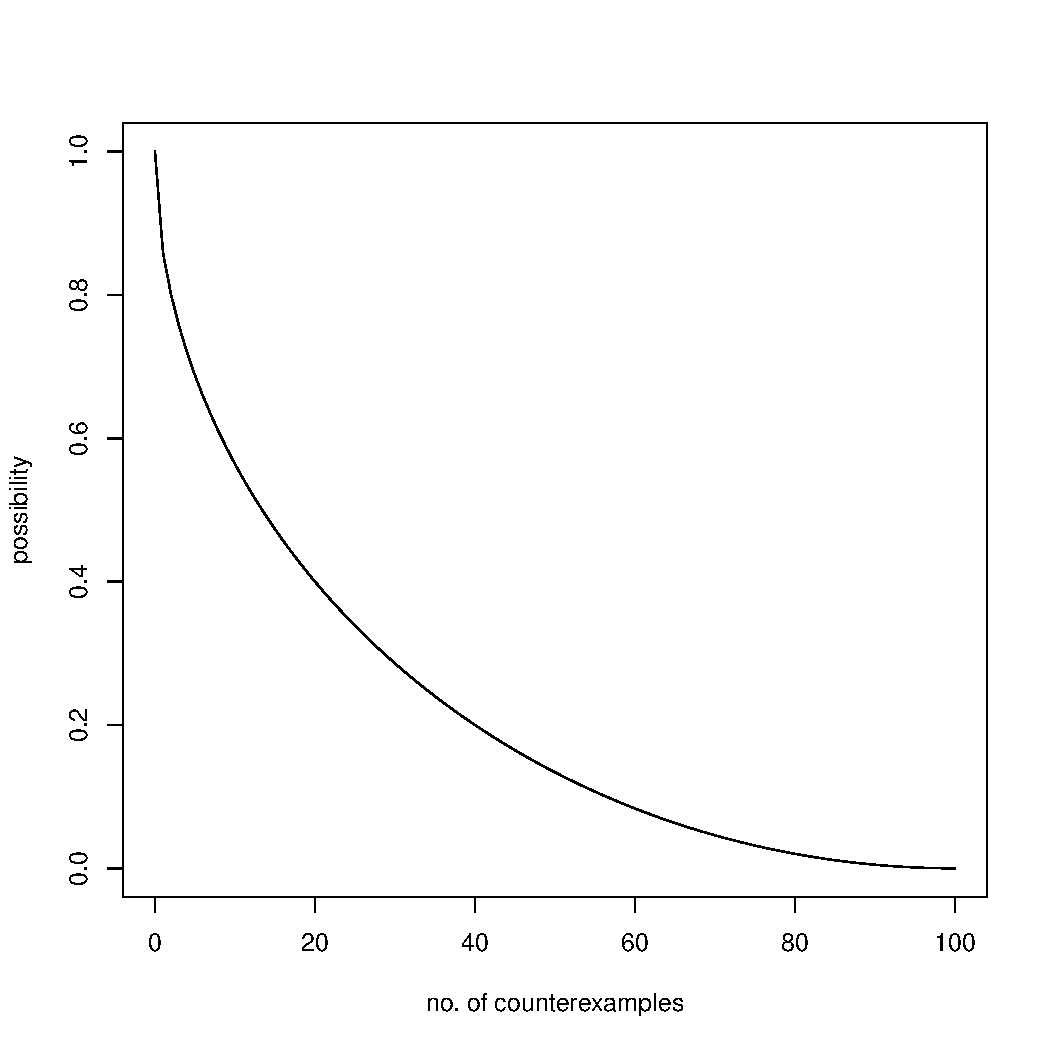
\includegraphics[width=2.25in]{../possibility} &
%      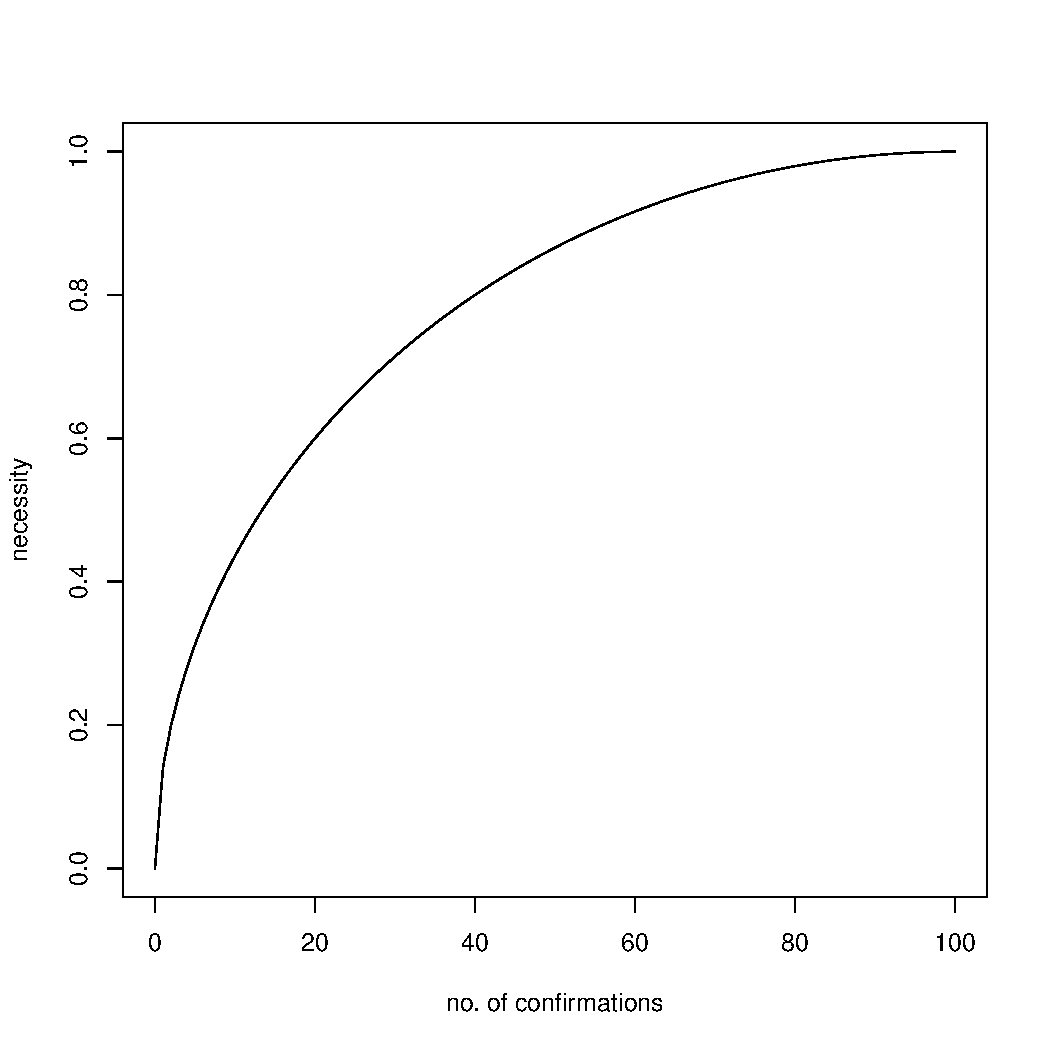
\includegraphics[width=2.25in]{../necessity} \\
%      (a) & (b)
%    \end{tabular}
%  \end{center}
%  \caption{A plot of $\Pi(\phi)$  as a function of
%    $u_\phi^-$ (a) and of $N(\phi)$ as a function of
%    $u_\phi^+$ (b) when $u_\phi = 100$.\label{fig:poss-nec-plots}}
%\end{figure}

\subsection{Axiom Scoring}
We combine the possibility and necessity of an axiom to define
a single handy acceptance/rejection index (ARI) as follows:
\begin{equation}\label{eq:ARI}
  \mathrm{ARI}(\phi) = N(\phi) - N(\neg\phi) = N(\phi) + \Pi(\phi) - 1 \in [-1, 1].
\end{equation}
A negative $\mathrm{ARI}(\phi)$ suggests rejection of $\phi$ ($\Pi(\phi)<1$),
whilst a positive $\mathrm{ARI}(\phi)$ suggests its acceptance ($N(\phi)>0$),
with a strength proportional to its absolute value. A value close to zero
reflects ignorance about the status of $\phi$.

\section{A Framework for Candidate Axiom Testing}
\label{OWL2SPARQL} 


However, unlike interpretation domains, RDF stores are incomplete and possibly noisy. 
%reviewer 4:
%What does incompleteness mean when talking about an interpretation means?
%cath: tjs le même pb...
To learn axioms from an RDF dataset, the open-world hypothesis must be made: the absence of
supporting evidence does not necessarily contradict an axiom, and an axiom might
hold even in the face of a few counterexamples.
For example, for 143 out of 541 \texttt{SubClassOf} axioms in the DBpedia
ontology, no resource in the DBpedia dataset provides any evidence;
for 28, at least one counterexample is found in DBpedia 3.9.
Axiom \texttt{SubClassOf(dbo:Person dbo:Agent)} even has 76 counterexamples!

%The semantics of the 32 axiom types of OWL~2 may be taken as a starting point to define,
%for each axiom type, which facts recorded in a given RDF triple store are to be taken as
%supporting evidence, or \emph{confirmations} of the axiom and which facts are to be
%construed as refuting evidence, or \emph{counterexamples}, based on the principles
%laid out in Section~\ref{epistemology}.

A general algorithm for testing all the possible OWL~2 axioms in a given RDF store is beyond the scope of this paper. 
Here, we will restrict our attention to \texttt{Class} and \texttt{ObjectComplementOf} class expressions and to \texttt{SubClassOf} axioms. Scoring these axioms with their ARI requires to compute the interpretation of \texttt{Class} and \texttt{ObjectComplementOf} class expressions. 

\subsection{Computational Definition of the Interpretation of \texttt{Class} and \texttt{ObjectComplementOf} Class Expressions}
We define a mapping $Q(E, \mbox{\tt ?x})$ from OWL~2 class expressions to SPARQL graph patterns,
where $E$ is an OWL~2 class expression, and $\mbox{\tt ?x}$ is a SPARQL variable,
%and match a resource identifier, or a literal,
%Cath est-ce qu'il n'y aurait pas des cas où on veut pouvoir matcher des blank nodes dans le cas général?
such that the query
\texttt{SELECT DISTINCT ?x WHERE \{} $Q(E, \mbox{\tt ?x})$ \texttt{\}}
returns all the individuals which are instances of $E$, which we will denote by
$[Q(E, \mbox{\tt ?x})]$. % and use to construct $E^\mathcal{I}$. 


For a \texttt{Class} class expression $A$ (i.e., an atomic concept in Description Logics (DL)), $Q(A, \mbox{\tt ?x}) = \mbox{\tt ?x a }A$,
where $A$ is a valid IRI.
For an \texttt{ObjectComplementOf} class expression, things are slightly more complicated, since RDF does not support
negation. The model-theoretic semantics of class expressions of the form \texttt{ObjectComplementOf(}$C$\texttt{)}
($\neg C$ in DL syntax), where $C$ denotes a class, is $\Delta^\mathcal{I} \setminus C^\mathcal{I}$.
The obvious definition
\begin{equation}\label{eq:neg-as-failure}
  Q(\neg C, \mbox{\tt ?x}) = 
  \begin{minipage}[t]{3in}
    \begin{tabbing}
      \quad\=\quad\=\quad\=\kill
      \{\>\texttt{?x ?p ?o .}\\
        \>\texttt{FILTER NOT EXISTS} $Q(C, \mbox{\tt ?x})$ \},
    \end{tabbing}
  \end{minipage}
\end{equation}
has the problem of treating negation as failure, like in databases,
where the closed-world assumption is made. 
Since we want to preserve an open-world semantics, $Q(\neg C, \mbox{\tt ?x})$ should be defined
differently, as the union of the concepts that are disjoint from $C$.
One might try to express this as the set of individuals $x$ that are instances of a
concept $C'$ such that no individual $z$ such that $C(z)$ is an instance of $C'$,
yielding the query
\begin{equation}\label{eq:approx-open-world-negation}
  Q(\neg C, \mbox{\tt ?x}) =
  \begin{minipage}[t]{3in}
    \begin{tabbing}
      \quad\=\quad\=\quad\=\kill
      \{\>\texttt{?x a ?dc .}\\
        \>\texttt{FILTER NOT EXISTS} \{\\
        \>\>\texttt{?z a ?dc . } $Q(C, \mbox{\tt ?z})$ \texttt{\} \}},
    \end{tabbing}
  \end{minipage}
\end{equation}
where \texttt{?z} is a variable that does not occur anywhere else in the query.
This translation is conceptually more satisfactory than the one in Equation~\ref{eq:neg-as-failure},
but it just pushes the problem one step further, because this way of testing whether
two concepts are disjoint is based on negation as failure too.
The only way to be certain that two classes are disjoint would be to find an axiom to
this effect in the ontology:
\begin{equation}\label{eq:negation-with-disjointWith}
  Q(\neg C, \mbox{\tt ?x}) =
  \begin{minipage}[t]{3in}
    \begin{tabbing}
      \quad\=\quad\=\quad\=\kill
      \{\>\texttt{?x a ?dc .}\\
        \>\texttt{?dc owl:disjointWith} $C$ \},
    \end{tabbing}
  \end{minipage}
\end{equation}
otherwise, either we find an individual which is an instance of both classes,
and thus we know the two classes are not disjoint, or we do not,
in which case the two classes may or may not be disjoint.
The fact is, very few \texttt{DisjointClasses} axioms are currently found in existing
ontologies. For example, in the DBpedia ontology, the query:\\
\texttt{SELECT ?x ?y \{ ?x owl:disjointWith ?y \}},\\ executed on November 22, 2013
returned 17 solutions only.
%TODO update the date of the execution
%Furthermore, we can write a query like the one in Equation~\ref{eq:negation-with-disjointWith}
%only if $C$ is an atomic concept! The definition cannot be extended to complex concepts
%because $C$ appears directly in the graph pattern, not inside a construct of the form
%$Q(C, \cdot)$, which would make induction work.

\begin{figure}[t!]
  \begin{center}
    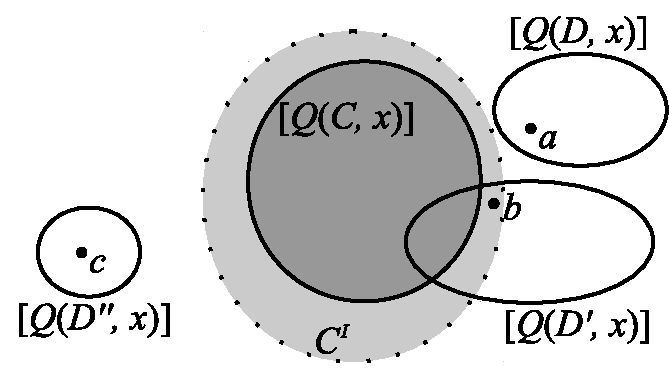
\includegraphics[height=1.4in]{../negation}
  \end{center}
  \caption{A schematic illustration of the heuristics used to capture negation
    under the open world assumption. $D''$ is a concept which is declared to
    be disjoint with $C$ in the RDF repository.\label{fig:negation}}
\end{figure}

To compare these three alternative definitions of $Q(\neg C, \mbox{\tt ?x})$,
we may refer to the diagram in Figure~\ref{fig:negation}. We wish to estimate
the actual extension of $\neg C$. Clearly, $Q(C, \mbox{\tt ?x})$
(in dark grey) underestimates the real extension of $C$ (in light gray).
Therefore, we may say that Equation~\ref{eq:neg-as-failure} overestimates
the real extension of $\neg C$,
in the sense that it will regard as instances of $\neg C$ all individuals $a$
for which ``$a \mbox{\tt\ a } C$'' is not found in the RDF repository.

Now, if $b$ is such that ``$b \mbox{\tt\ a } C$'' is not known, but ``$b \mbox{\tt\ a } D'$''
is known for some class $D'$ and some instances of $D'$ are known to be also
instances of $C$, then it might well be that $b$ is an instance of $C$ as well.
If, however $a$ is such that ``$a \mbox{\tt\ a } C$''
is not known, but ``$a \mbox{\tt\ a } D$'' is known for some class $D$ but
no instance of $D$ is known that is also an instance of $C$, then we are more
likely to believe that $a$ is not an instance of $C$.
Therefore Equation~\ref{eq:approx-open-world-negation} regards as instances of $\neg C$
fewer individuals, those for which it is highly likely that they do not belong
to $C$. It might still overestimate the extension of $\neg C$, but much less
than Equation~\ref{eq:neg-as-failure}. In fact, it might even underestimate it,
as far as we know.

On the other hand, it is certain that Equation~\ref{eq:negation-with-disjointWith}
will underestimate the extension of $\neg C$, to the point that it will equate it
with the empty set if no triple of the form ``$D''$ \texttt{owl:disjointWith} $C$''
is declared in the RDF repository. Furthermore, it might well be that an individual
is an instance of $\neg C$ even though it is not an instance of an atomic class disjoint with $C$!

To sum up, Equation~\ref{eq:approx-open-world-negation} looks like a sensible
compromise between Equation~\ref{eq:neg-as-failure} (too optimistic)
and Equation~\ref{eq:negation-with-disjointWith} (too pessimistic).
%reviewer 5: the choice of the right equation deserve an empirical study
%TODO: c'est une très bonne idée!!!

We will end this section by arguing that a suitable definition of confirmation to adopt in this
framework is Scheffler and Goodman's \emph{selective confirmation}~\cite{SchefflerGoodman1972},
which characterizes a confirmation as a fact not simply satisfying an axiom, but, further,
favoring the axiom rather than its contrary.
For instance, the occurence of a black raven \emph{selectively confirms} the axiom
$\mathtt{Raven} \sqsubseteq \mathtt{Black}$ because it both confirms it and fails to confirm its
negation, namely that there exist ravens that are not black. On the contrary, the observation of
a green apple does not contradict $\mathtt{Raven} \sqsubseteq \mathtt{Black}$,
but it does not disconfirm $\mathtt{Raven} \not\sqsubseteq \mathtt{Black}$
either; therefore, it does not selectively confirm $\mathtt{Raven} \sqsubseteq \mathtt{Black}$.
We will incorporate this principle in our computational
definition of a confirmation in Section~\ref{comp-def-ARI} below.


\subsection{Computational Definition of the Content of \texttt{SubClassOf} Axioms}

The semantics of \texttt{SubClassOf} axioms of the form $C~\sqsubseteq~D$ in DL syntax is $C^\mathcal{I} \subseteq D^\mathcal{I}$,
which may also be written $x \in C^\mathcal{I} \Rightarrow x \in D^\mathcal{I}$. 
The content of such axioms may thus be defined as
\begin{equation}
  \mathrm{content}(C \sqsubseteq D) = \{D(a) : \mbox{$C(a)$ in the RDF store} \},
\end{equation}
because, if $C(a)$ holds, then
\[
  C(a) \Rightarrow D(a) \equiv \neg C(a) \lor D(a) \equiv \bot \lor D(a) \equiv D(a).
\]
The support $u_{C \sqsubseteq D}$ of such axioms can be computed with the following SPARQL query:
\begin{equation}
  \begin{minipage}[c]{5in}
    \begin{tabbing}
      \quad\=\quad\=\quad\=\kill
      \texttt{SELECT (count(DISTINCT ?x) AS ?u)}\\
      \texttt{WHERE} \{$Q(C, \mbox{\tt ?x})$\}.
    \end{tabbing}
  \end{minipage}
\end{equation}

\subsection{Computational Definition of the ARI of \texttt{SubClassOf} Axioms}
\label{comp-def-ARI}

In order to compute $ARI(C \sqsubseteq D)$, we must provide a computational definition of $u^+_{C \sqsubseteq D}$ and $u^-_{C \sqsubseteq D}$. We start with the following statements:
\begin{itemize}
\item confirmations are individuals $i$ such that\\
  $i \in [Q(C, \mbox{\tt ?x})]$ and $i \in [Q(D, \mbox{\tt ?x})]$;
\item counterexamples are individuals $i$ such that\\
  $i \in [Q(C, \mbox{\tt ?x})]$ and $i \in [Q(\neg D, \mbox{\tt ?x})]$.
\end{itemize}
This may be translated into the following two SPARQL queries to compute $u^+_{C \sqsubseteq D}$ and $u^-_{C \sqsubseteq D}$ respectively:
\begin{equation}
  \begin{minipage}[c]{5in}
    \begin{tabbing}
      \quad\=\quad\=\quad\=\kill
      \texttt{SELECT (count(DISTINCT ?x) AS ?nConfirm)}\\
      \texttt{WHERE} \{ $Q(C, \mbox{\tt ?x})$ $Q(D, \mbox{\tt ?x})$ \}
    \end{tabbing}
  \end{minipage}
\end{equation}
and
\begin{equation}
  \begin{minipage}[c]{5in}
    \begin{tabbing}
      \quad\=\quad\=\quad\=\kill
      \texttt{SELECT (count(DISTINCT ?x) AS ?nCounter)}\\
      \texttt{WHERE} \{ $Q(C, \mbox{\tt ?x})$ $Q(\neg D, \mbox{\tt ?x})$ \}.
    \end{tabbing}
  \end{minipage}
\end{equation}
Notice that an $i$ such that $i \in [Q(C, \mbox{\tt ?x})]$ and $i \notin [Q(D, \mbox{\tt ?x})]$
does not contradict $C \sqsubseteq D$, because it might well be the case
that the assertion ``$i \mbox{\tt\ a } D$'' is just missing.
Likewise, an $i \in [Q(\neg D, \mbox{\tt ?x})]$ such that $i \in [Q(\neg C, \mbox{\tt ?x})]$
will not be treated as a confirmation, based on our choice to regard as
evidence in favor of a hypothesis only selective confirmations.



\subsection{Heuristics based on Time Capping}

The results of our first experimentation described in the following Section~\ref{evaluation}
show that the time it takes to test an axiom tends to be upper bounded by the inverse
of $1 + \mathrm{ARI}(\phi)$: an axiom which takes too long to test will likely end up having a very negative score.
We defined two heuristics based on this idea.
\begin{itemize}
\item We time-cap the SPARQL queries to compute the ARI of a candidate axiom and decide whether to accept or reject it, since above a computation time threshold, the axiom being tested is likely to get a negative ARI and be rejected.
\item We construct candidate axioms of the form $C \sqsubseteq D$, by considering
the subclasses $C$ in increasing order of the number of classes $D$ sharing at least
one instance with $C$.
This enables us to maximize the number of tested and accepted axioms in a given time period,
since it appears that the time it takes to test $C \sqsubseteq D$ increases with that number
and the lower the time, the higher the ARI.
\end{itemize}

%In statistics, \emph{censoring} is when the value of a measurement or observation
%is not known for some sample points. A sample contains censored observations
%if the only information about some of the observations is that they are below
%or above a specified value.
%
% NIST/SEMATECH e-Handbook of Statistical Methods, http://www.itl.nist.gov/div898/handbook/, Jan 11, 2015
% http://www.itl.nist.gov/div898/handbook/apr/section1/apr131.htm
%
% Chapter 11, Analyzing Below Detection-limit data, from Millard, Dixon, and Neerchal, Environmental Statistics with R
% http://www.public.iastate.edu/~pdixon/stat505/Chapter%2011.pdf

%Here, we use this concept to refer to the fact that, when testing an OWL axiom,
%if one caps the time the test should take, the exact value of the score
%for the axiom whose test times out will not be known.
%From a statistical point of view, this produces a random censoring,
%because both the number of censored observations and the censoring levels
%are random outcome.

\section{Evaluation on \texttt{SubClassOf} Axiom Testing}
\label{evaluation}

%reviewer 1
%it is not really clear how the accuracy was measured (i.e., why the proposed ARI index is more accurate than the probabilistic score) 


\subsection{Experimental Protocol}

We evaluated the proposed scoring heuristics by performing tests of subsumption
axioms using DBpedia 3.9 in English as the reference RDF fact repository.
In particular, on April 27, 2014, we downloaded the DBpedia dumps of English version 3.9,
generated in late March/early April 2013, along with the DBpedia ontology, version 3.9.
This local dump of DBpedia, consisting of 812,546,748 RDF triples,
has been bulk-loaded into Jena TDB and a prototype
for performing axiom tests using the proposed method has been coded in Java,
using Jena ARQ and TDB to access the RDF repository.

We systematically generated and tested subsumption axioms
involving atomic classes only according to the following protocol:
for each of the 442 classes $C$ referred to in the RDF repository,
we construct all axioms of the form $C \sqsubseteq D$ such that $C$ and $D$
share at least one instance. Classes $D$ are obtained with the following query: 


\begin{minipage}[c]{5in}
    \begin{tabbing}
      \quad\=\quad\=\quad\=\kill
      \texttt{SELECT DISTINCT ?D}\\
      \texttt{WHERE \{}$Q(C, \mbox{\tt ?x})$ . \texttt{?x a ?D\}}.
    \end{tabbing}
  \end{minipage}


Experiments have been performed on two machines:
\begin{itemize}
\item a Fujitsu CELSIUS workstation equipped
with twelve six-core Intel Xeon CPU E5-2630 v2 processors at 2.60GHz clock speed,
with 15,360 KB cache each, 128 GB RAM,
4 TB of disk space with a 128 GB SSD cache,
under the Ubuntu  12.04.4 LTS 64-bit operating system;
\item a HP  portable PC equipped
% according to the /proc/cpuinfo file on TOMTY
with four two-cores Intel\textregistered\ Core\texttrademark\ i7-4600U CPUs at 2.10GHz clock speed,
with a 4,096 KB cache, 16 GB RAM,
128 GB of disk space,
under the Fedora 64-bit Linux operating system.
\end{itemize}
The former was used to test 644 axioms without time capping.
The latter, much less powerful but representative of a common high-end laptop computer,
was then used to obtain the results with time capping.




\subsection{Results without Time Capping}
\label{results-no-timeout}

We managed to test 644 axioms without time capping.
Figure~\ref{fig:ARI-BLS} compares the results obtained in this preliminary experiment
to the probabilistic score proposed in~\cite{BuehmannLehmann2012}.
As already discussed in~\cite{TettamanziFaronZuckerGandon2014ekaw}, the proposed
acceptance-rejection index is more accurate than the probabilistic score.
However, its increased accuracy comes at a higher computational cost.
The two heuristics, time capping and candidate axioms ordering, make up for it.

%Cath ne pas faire référence aux couleurs dans les explications de graphiques car impressions noir et blanc

\begin{figure}[t]
\begin{center}
    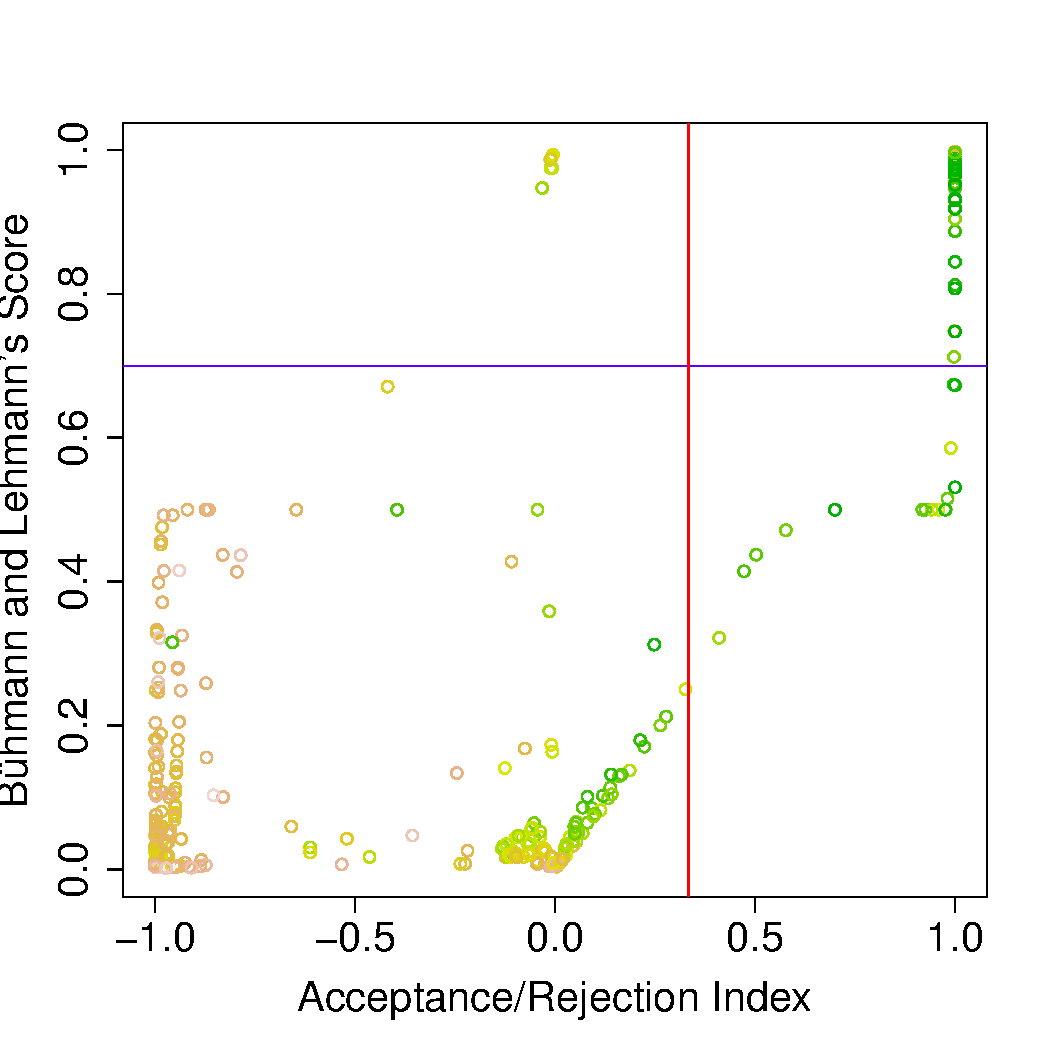
\includegraphics[height=2.5in]{ARI-BLS}
\end{center}
\caption{A comparison of the acceptance/rejection index and the probability-based
  score used in~\cite{BuehmannLehmann2012} on axioms tested without time capping.
  The vertical line shows the acceptance threshold $\mathrm{ARI}(\phi)>1/3$;
  the horizontal line the acceptance threshold of 0.7 for the probabilistic score.}
\label{fig:ARI-BLS}
\end{figure}

\begin{figure}[t]
\begin{center}
    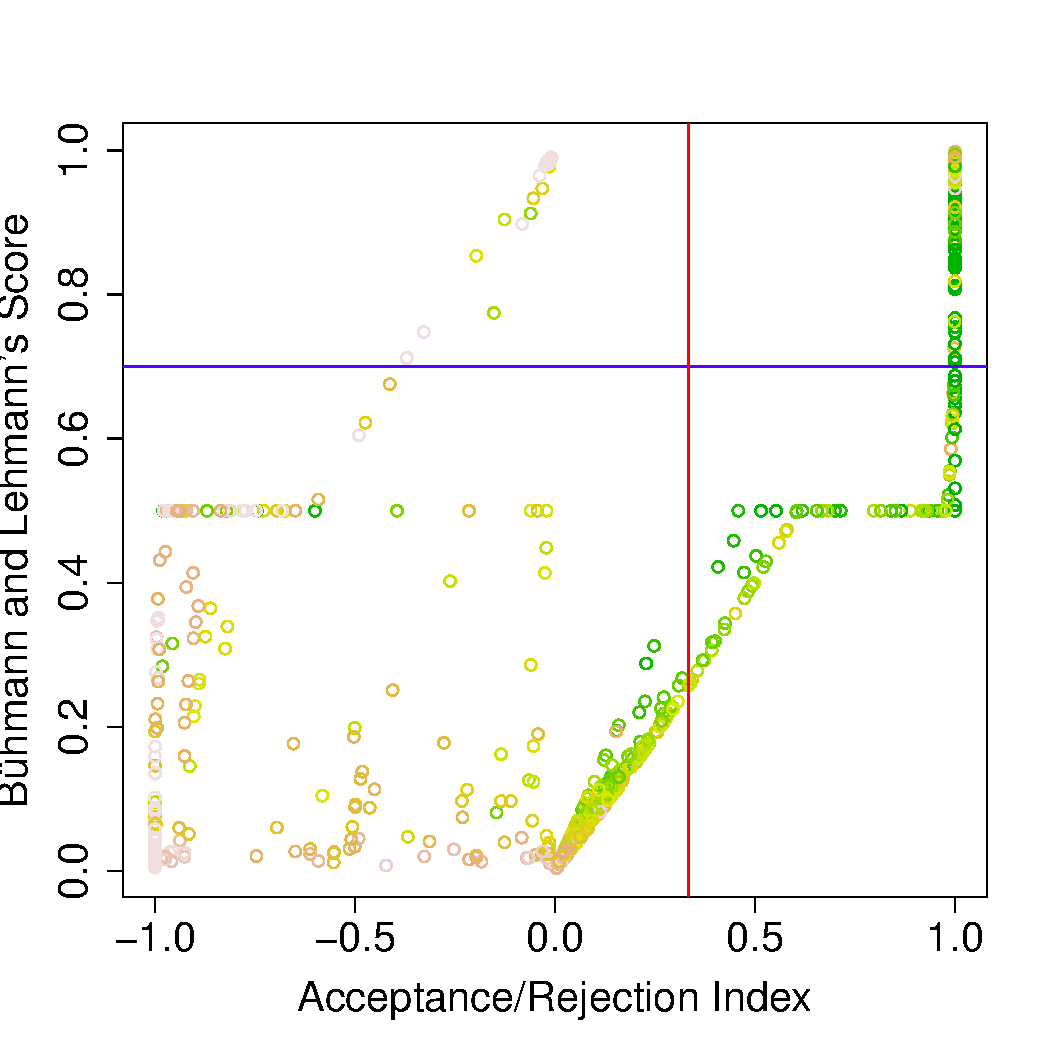
\includegraphics[height=2.5in]{ARI-BLS-20}
\end{center}
\caption{A comparison of the acceptance/rejection index and the probability-based
  score used in~\cite{BuehmannLehmann2012} on axioms tested with a 20-minute time cap.
  The vertical line shows the acceptance threshold $\mathrm{ARI}(\phi)>1/3$;
  the horizontal line the acceptance threshold of 0.7 for the probabilistic score.}
\label{fig:ARI-BLS-20}
\end{figure}


\begin{figure}[t]
\begin{center}
  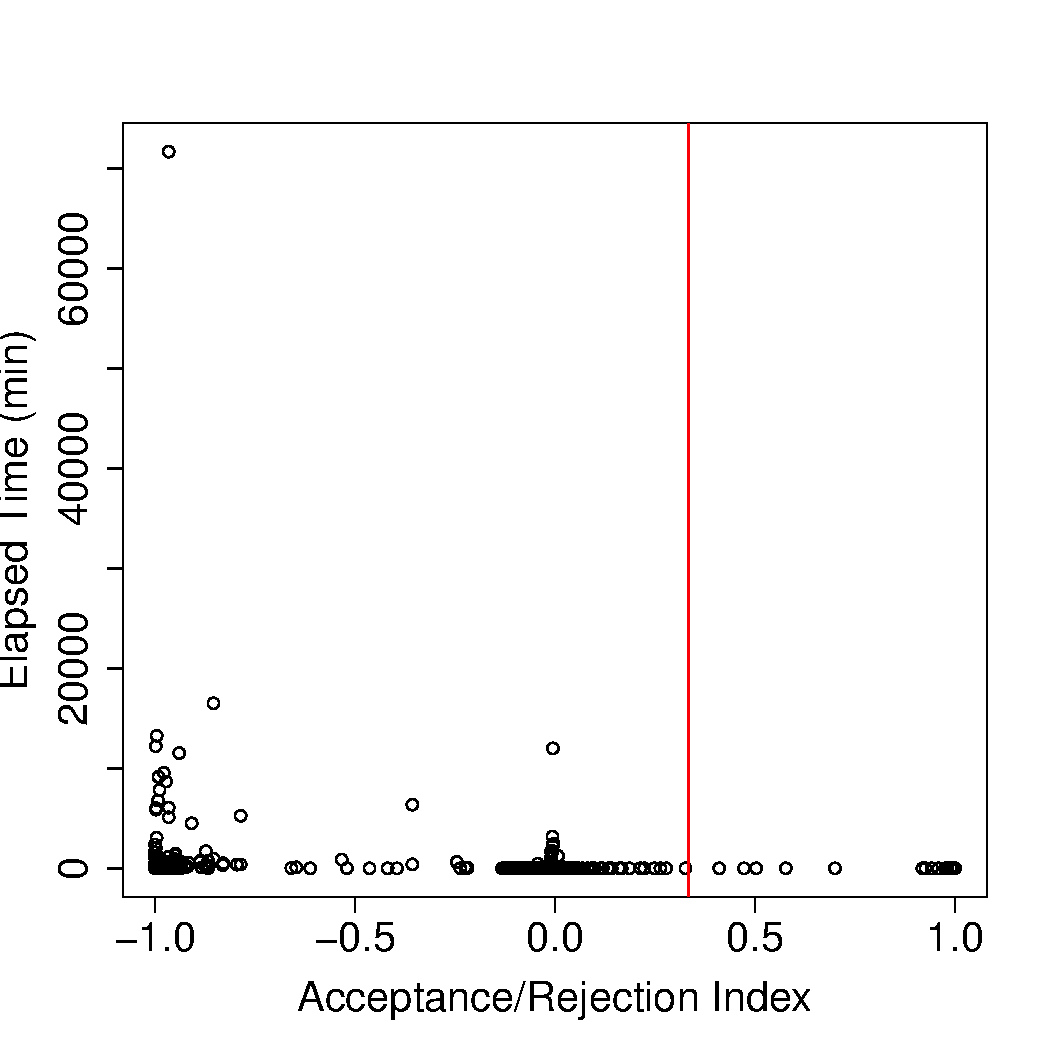
\includegraphics[height=2.5in]{time-ARI}
\end{center}
\caption{Plot of the time taken for testing the systematically generated
 \texttt{SubClassOf} axioms without time capping as a function of ARI.
  The vertical line shows the acceptance threshold $\mathrm{ARI}(\phi)>1/3$.}
\label{fig:time-ARI}
\end{figure}

%\begin{figure}[t]
%\begin{center}
%    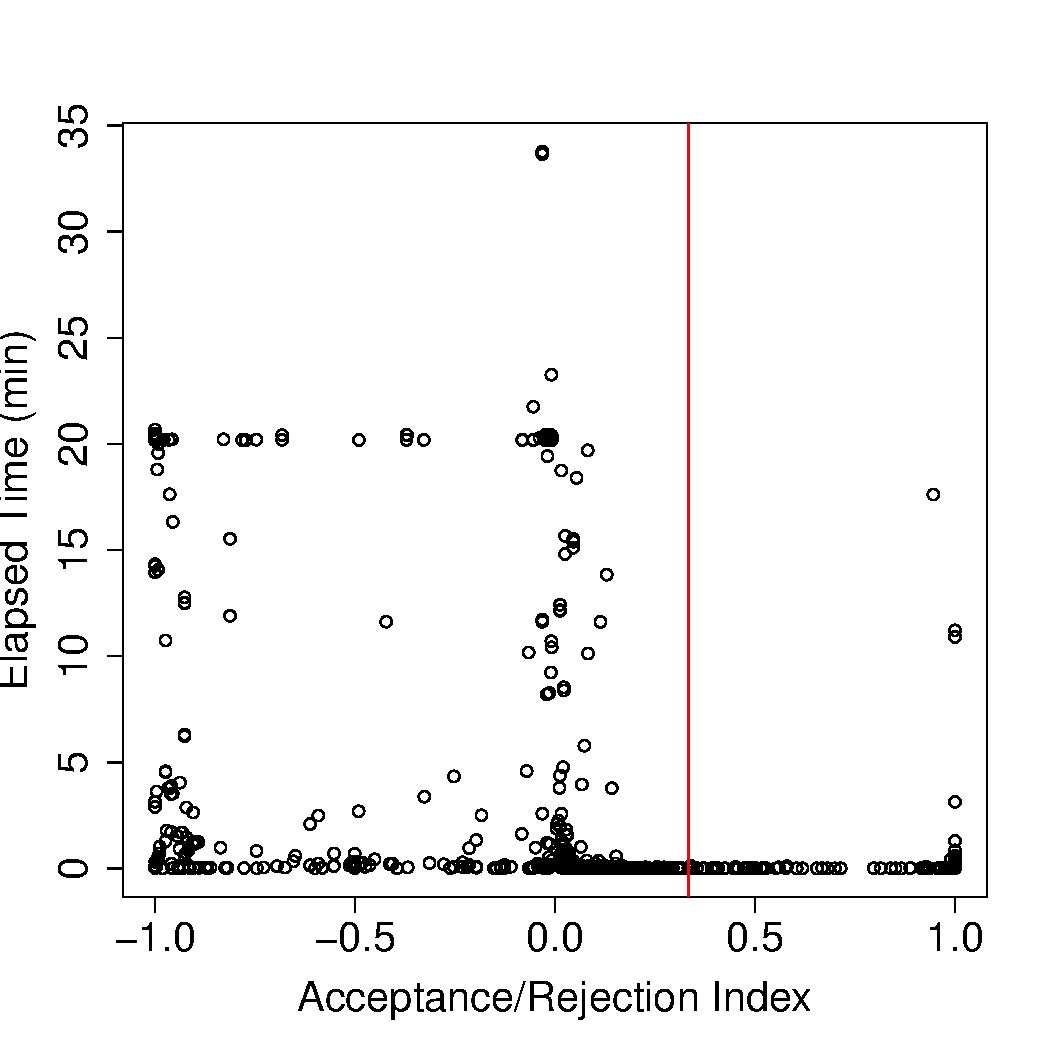
\includegraphics[height=2.5in]{time-ARI-20}
%\end{center}
%\caption{Plot of the time taken for testing the systematically generated
% \texttt{SubClassOf} axioms with a 20-minute time cap as a function of ARI.
%  The vertical line shows the acceptance threshold $\mathrm{ARI}(\phi)>1/3$.}
%\label{fig:time-ARI-20}
%\end{figure}

The results of this first experiment
show that the time it takes to test an axiom tends to be inversely proportional
to its score (see Figure~\ref{fig:time-ARI}): an axiom which takes
too long to test will likely end up having a very negative score.
If we restrict our attention to the 197 axioms with an ARI above the
acceptance threshold empirically set at $1/3$ in~\cite{TettamanziFaronZuckerGandon2014ekaw},
we discover that the average elapsed time for testing them is 20.5~s,
the median time is 156~ms, and the longest elapsed time is 1584.3~s, or 26~min 24~s.
Out of the 197 accepted axioms,
135 (68.5\%) were tested in less than 1~s,
165 (83.75\%) in less than 10~s,
187 (95\%) in less than 1~minute,
and 195 (99\%) in less than 10~minutes.

Altogether, testing those 644 axioms took a staggering 20,328,791,473~ms (= 235~days 6~h 53~min 11.473~s).
If all tests had been time-capped to exactly 10 minutes, the total elapsed time
would have been ``just'' 182,481,760~ms (= 2 days 2~h 41~m 21.76~s),
i.e., less than 0.9\% of the actual time, with a two orders of magnitude speedup!


% THE FOLLOWING IS COMMENTED OUT, BECAUSE IT WILL BE DISCUSSED IN THE ISWC PAPER
%More precisely the time it takes to test a \texttt{SubClassOf} axiom of the form
%$C \sqsubseteq D$ is proportional to the product of the cardinality of $C$
%and the number of classes that have at least a known instance in common with $C$,
%as shown in Figure~\ref{fig:time-tp}. We will call this product the \emph{time predictor}.



\subsection{Results with Time Capping}

Based on these observations, we decided to fix to 20 min
(i.e., twice the time it took to test 99\% of the accepted axioms on the more powerful machine)
the threshold to time-cap the SPARQL queries to compute $u^+_{C \sqsubseteq D}$ and $u^-_{C \sqsubseteq D}$
in order to decide whether to accept or reject a candidate axiom $C \sqsubseteq D$.

For this new round of experiments, we used the candidate axiom ordering heuristics
in order to get as much tested axioms as possible.
Thanks to the greatly reduced overhead, %(cf.\ Figure~\ref{fig:time-ARI-20}),
we were able to test 3,530 axioms at the time of writing.
The results are shown in Figure~\ref{fig:ARI-BLS-20}.

%%Cath: J'ai intégré cela dans l'analyse qualitative
%There are 98 axioms that were tested both with and without time capping;
%the outcome of the test is different on just four of them,
%namely:\\
%\texttt{dbo:Road}~$\sqsubseteq$~\texttt{gml:\_Feature},\\
%\texttt{dbo:Library}~$\sqsubseteq$~\texttt{gml:\_Feature},\\
%\texttt{schema:School}~$\sqsubseteq$~\texttt{dbo:Agent}, and \\
%\texttt{schema:School}~$\sqsubseteq$~\texttt{gml:\_Feature}.\\
%That represents an error rate of 4.1\%. If we take into account the dramatic
%improvement in terms of speed, this looks like a very reasonable price to pay
%in terms of accuracy degradation. In addition, it should be observed that,
%by construction, the errors are all in the same direction, i.e., some axioms
%which should be accepted are in fact rejected: at least, this is a conservative
%heuristics, since it does not generate false positives.

%\begin{figure}[t]
%\begin{center}
%  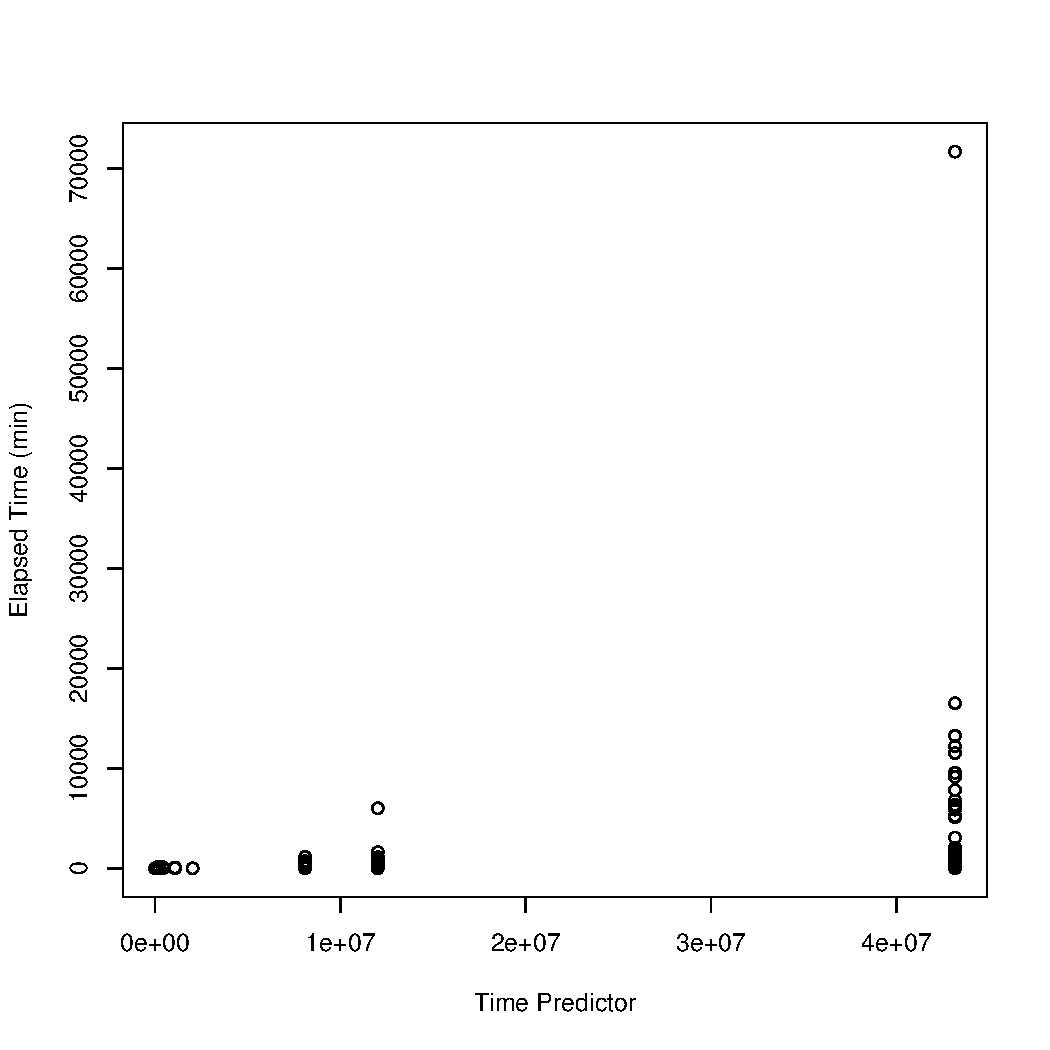
\includegraphics[height=2.5in]{time-tp}
%\end{center}
%\caption{Plot of the time taken to test all axioms (accepted and rejected)
%  as a function of the time predictor.}
%\label{fig:time-tp}
%\end{figure}

%\begin{figure}[t]
%\begin{center}
%  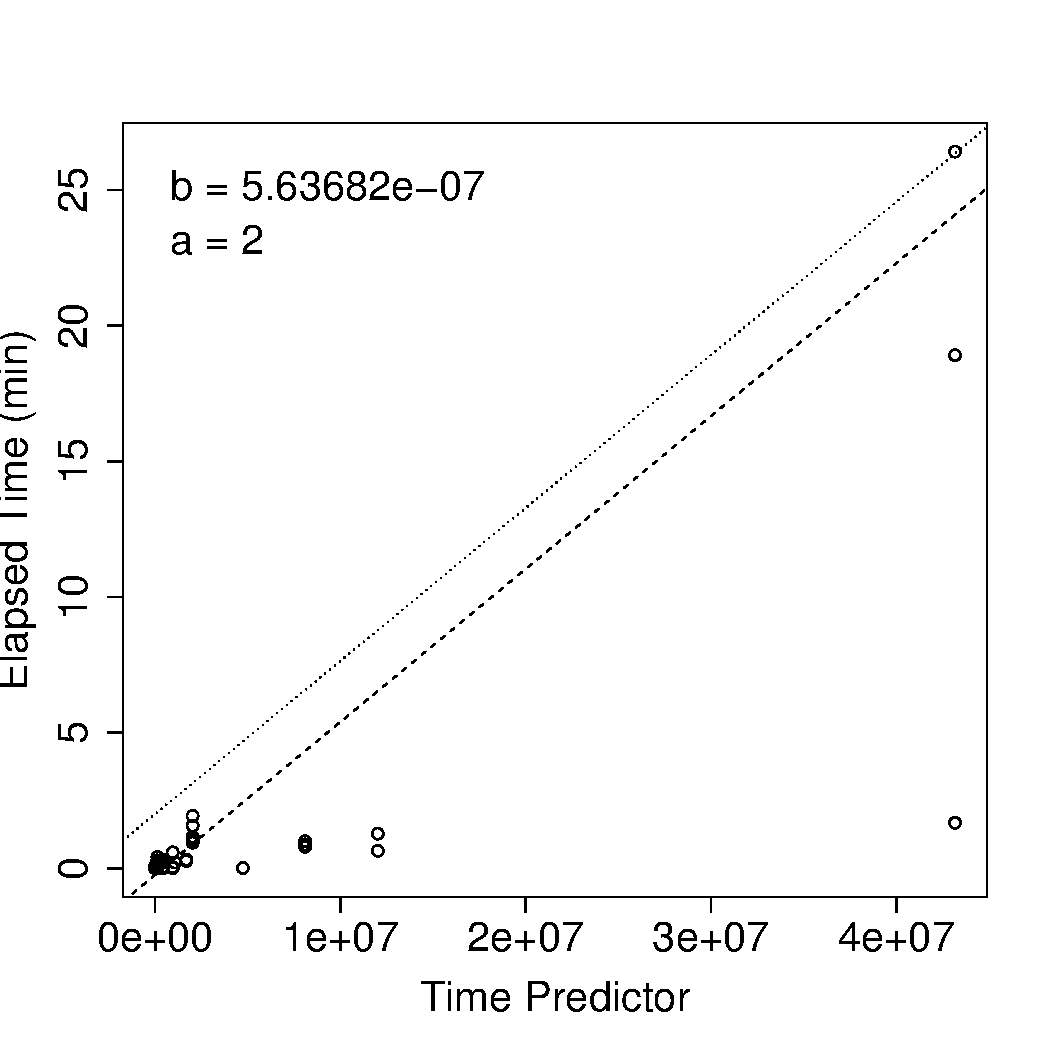
\includegraphics[height=2.5in]{time-tp-acc}
%\end{center}
%\caption{Plot of the time taken to test the accepted axioms as a function of the time predictor.}
%\label{fig:time-tp-acc}
%\end{figure}

%\begin{figure}[t]
%\begin{center}
%  \begin{tabular}{cc}
%    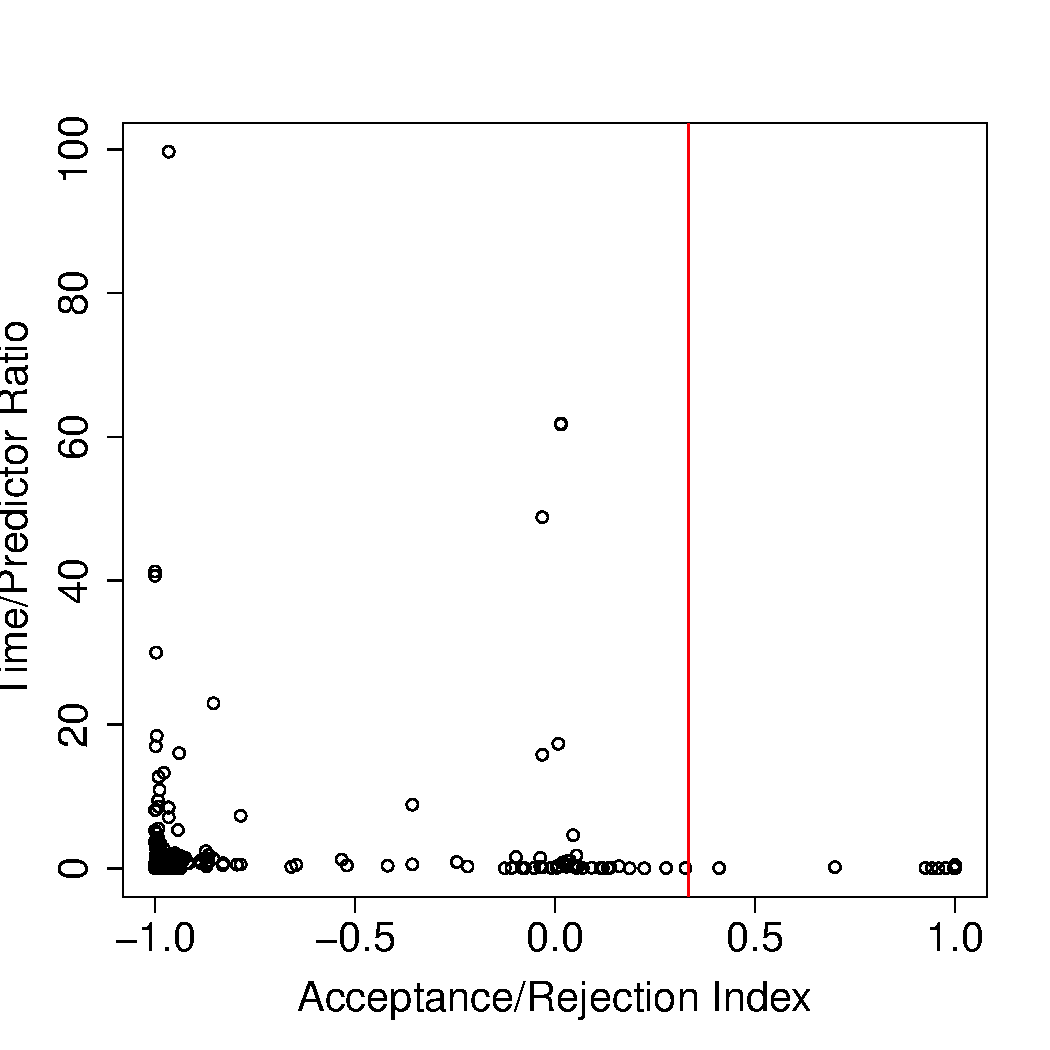
\includegraphics[height=2.25in]{ratio-ARI} &
%    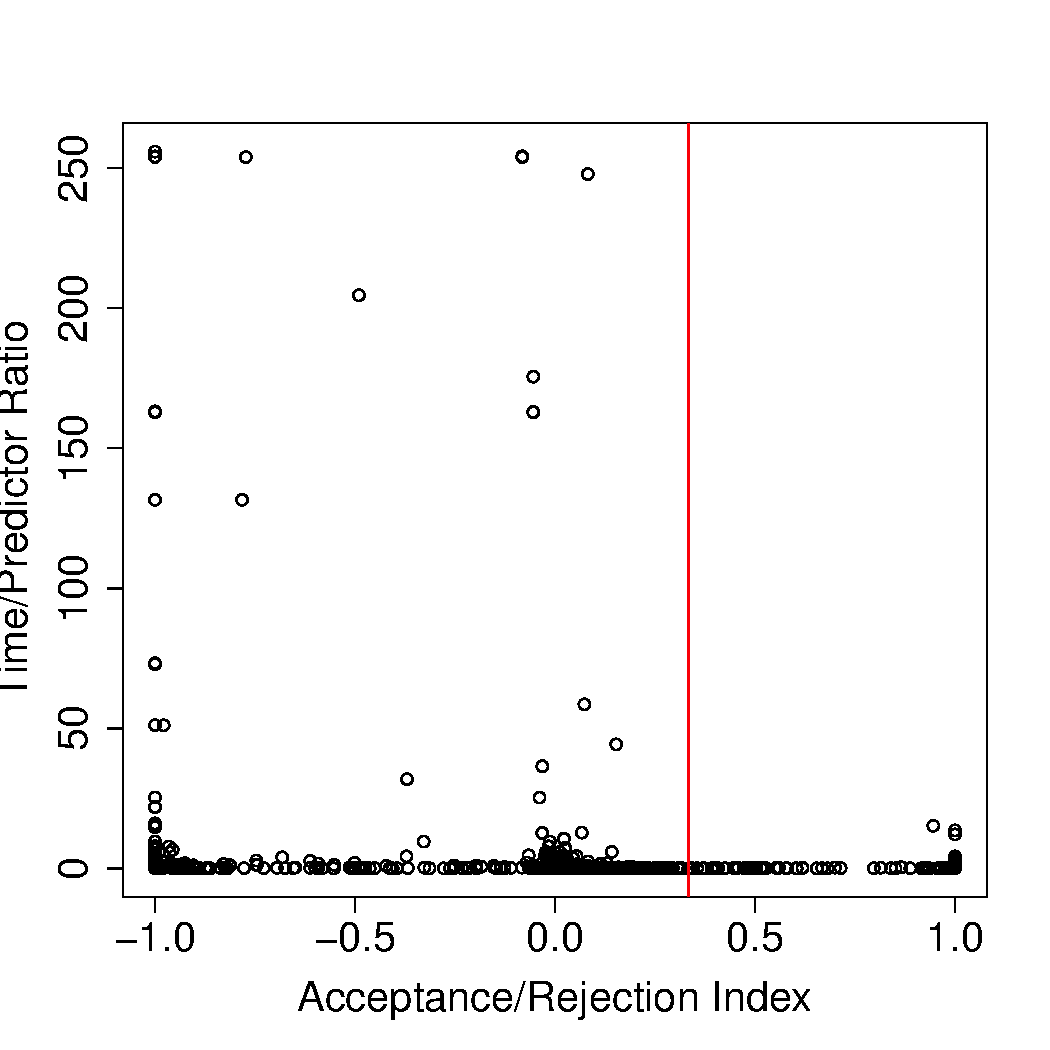
\includegraphics[height=2.25in]{ratio-ARI-20} \\
%    (a) & (b)
%  \end{tabular}
%\end{center}
%\caption{Plots showing the ratio of the time taken to test the axioms to the predictor
%  as a function of their acceptance-rejection index without time capping (a)
%  and with a 20-minute time cap (b).
%  The red line shows the acceptance threshold $\mathrm{ARI}(\phi)>1/3$.}
%\label{fig:ratio-ARI}
%\end{figure}

\subsection{Qualitative Analysis of the Results}
%TODO compare with the DBpedia ontology

A human analysis of the results of the automatic process shows that out of the 2426 candidate axioms which were tested, 204 are questionnable, i.e. $8.3\%$ of the results. 55 rejected axioms (scored by the system with an ARI value under the acceptance threshold) may be false negative and 149 accepted axioms (scored by the system with an ARI value above the acceptance threshold) may be false positive. 

The close analysis of the possibly 55 false positive led to the following conclusions:
\begin{itemize}
\item 44 of them are time-capped axioms. That represents an error rate of 1.8\%. If we take into account the dramatic
improvement in terms of speed, this looks like a very reasonable price to pay
in terms of accuracy degradation. In addition, it should be observed that,
by construction, the errors are all in the same direction, i.e., some axioms
which should be accepted are in fact rejected: at least, this is a conservative
heuristics, since it does not generate false positives.
\item Among the 11 remaining false positive, 4 of them have a positive ARI (under the acceptance threshold). This may lead to the reasonable conclusion that the candidate axioms rejected with a ARI close to the acceptance threshold should always be examined by an ontologist. The 7 remaining axioms involve very general classes as superclass, e.g., \texttt{dbo:Person}, \texttt{dbo:Product}. Their low scoring may be the result of incomplete knowledge due to the fact that people populating the DBpedia ontology will focus on more specific classes. 
\end{itemize}

Conversely, the analysis of the 148 possibly false positive led to the following conclusions:
\begin{itemize}
\item Most of these axioms which should be rejected are inverted \texttt{subClassOf} relations between concepts (e.g. \texttt{dbo:Case} $\sqsubseteq$ \texttt{dbo:LegalCase} instead of \texttt{dbo:LegalCase} $\sqsubseteq$ \texttt{dbo:Case}). This occurs when counterexamples are missing (all instances of a class are instances of the other class too and the two axioms are positively scored).
%other inverted subClassOf relations: between dbo:SportManager and SoccerManager, dbo:ClericalAdministrativeRegion and dbo:Diocese, dbo:Region and dbo:AdministrativeRegion

\item The acceptation of some axioms involving vague concepts is questionable. For instance, it seems that anything that can appear on a map could be typed with \texttt{gml:\_Feature} and therefore many classes should be subclasses of it, but it is not clear whether this is correct or not. The same remark applies to \texttt{SubclassOf} axioms with class \texttt{dbo:Place} as superclass.

\item Some axioms involve concepts used in a more general sense than it could be expected. Their acceptation is therefore dubious. It is for instance the case of \texttt{dbo:PokerPlayer}~$\sqsubseteq$~\texttt{dbo:Athlete}. Its acceptation is not really a mistake in the sense that there are several other such concepts involving \texttt{dbo:Athlete}, e.g. \texttt{dbo:FigureSkater}~$\sqsubseteq$~\texttt{dbo:Athlete}. These axioms are acceptable when considering \texttt{dbo:Athlete} in its general sense.

\item Other questionable axioms are those involving a concept having at least two senses, e.g \texttt{dbo:Library} designating both a building and an institution. The joint acceptation of axioms \texttt{schema:Library}~$\sqsubseteq$~\texttt{dbo:Organisation} and \texttt{schema:Library}~$\sqsubseteq$~\texttt{dbo:Place} is not satisfactory.

\item Other questionable axioms are those involving a concept both used as a zoological class name, a taxon, and therefore marked as subclass of \texttt{dbp:Species}, and as a set of animals, and therefore subclass of \texttt{dbo:Animal} and  \texttt{dbo:Eukaryote}. This is for instance the case of \texttt{dbo:Insect}.

\item The same confusion between the instance level and the ontological level explain that most of the axioms involving \texttt{skos:Concept} should be rejected, e.g., \texttt{dbo:Activity}~$\sqsubseteq$~\texttt{skos:Concept} or \texttt{dbo:Train}~$\sqsubseteq$~\texttt{skos:Concept}.

%pb de modélisation sur domaines de pointe: en biologie, en juridique (SupremeCourtOfTheUnitedStatesCase)

\end{itemize}
To sum up, the high scoring of most of the candidate axioms which should be rejected is due to misconceptions in the DBpedia RDF base, misuses of the DBpedia ontology by people populating it.
%TODO contrairement à ce qu'on pensait, ceux qui sont discutable ne sont pas forcément ceux avec peu de confirmations




\section{Conclusion}\label{conclusion}

We have presented a possibilistic axiom scoring heuristics which is a viable
alternative to statistics-based heuristics. We have tested it by applying it to the
problem of testing \texttt{SubClassOf} axioms against the DBpedia database.
We have also proposed additional heuristics to greatly reduce its computational
overhead, consisting of setting a time-out on the test of each axiom and ordering the candidate axioms according to their score in order to optimize the number of axioms tested in a given time period.

Our results, albeit preliminary, strongly support the validity of our hypothesis
that it is possible to alleviate the computation of the ARI without loosing too much
in terms of accuracy.

In addition, the qualitative analysis of the results confirm the interest of using axiom scoring heuristics like ours
not only to learn axioms from the LOD, but also to drive the validation and debugging of ontologies and RDF datasets.


%\section*{Acknowledgment}



% trigger a \newpage just before the given reference
% number - used to balance the columns on the last page
% adjust value as needed - may need to be readjusted if
% the document is modified later
%\IEEEtriggeratref{8}
% The "triggered" command can be changed if desired:
%\IEEEtriggercmd{\enlargethispage{-5in}}

% references section

\bibliographystyle{tetta-IEEEtran}
\bibliography{../RDFMining}

\end{document}


